% !TEX program = xelatex
\documentclass[11pt,a4paper]{article}

\usepackage[a4paper,margin=2.4cm,top=2.5cm,bottom=2.7cm]{geometry}
\usepackage{parskip}
\usepackage{microtype}
\usepackage{needspace}
\usepackage{enumitem}
\setlist{itemsep=2pt,topsep=4pt,parsep=0pt}

\usepackage{fontspec}
% Body font (per brand): Source Serif 4
\setmainfont{Source Serif 4}[
  Path=/sessions/loving-intelligent-shannon/.fonts/sourceserif/,
  Extension=.otf,
  UprightFont=SourceSerif4-Regular,
  ItalicFont=SourceSerif4-It,
  BoldFont=SourceSerif4-Bold,
  BoldItalicFont=SourceSerif4-BoldIt,
  Ligatures=TeX,
]
% Display font (per brand): Cormorant Garamond
\setsansfont{Cormorant Garamond}[
  Path=/sessions/loving-intelligent-shannon/.fonts/cormorant/,
  Extension=.ttf,
  UprightFont=CormorantGaramond-Regular,
  ItalicFont=CormorantGaramond-Italic,
  BoldFont=CormorantGaramond-Bold,
  BoldItalicFont=CormorantGaramond-BoldItalic,
  Ligatures=TeX,
]
% Cormorant Garamond Medium (used for the cover title per brand)
\newfontfamily\titlefont{Cormorant Garamond}[
  Path=/sessions/loving-intelligent-shannon/.fonts/cormorant/,
  Extension=.ttf,
  UprightFont=CormorantGaramond-Medium,
  ItalicFont=CormorantGaramond-MediumItalic,
  BoldFont=CormorantGaramond-Bold,
  BoldItalicFont=CormorantGaramond-BoldItalic,
  Ligatures=TeX,
]
\setmonofont{DejaVu Sans Mono}[Scale=0.78]

% =========================================================================
% BRAND COLOR PALETTE — Intelligent Internet
% Primary:   Sky Blue #bee6ed, Navy Blue #0f233f, Parchment #f2eee2
% Secondary: Periwinkle #83a1cc, Slate Grey #546070, Sea Foam #e8ede5,
%            Mist Grey #ebedee, Stone #808080
% =========================================================================
\usepackage{xcolor}
\definecolor{navy}{HTML}{0F233F}
\definecolor{periwinkle}{HTML}{83A1CC}
\definecolor{slate}{HTML}{546070}
\definecolor{parchment}{HTML}{F2EEE2}
\definecolor{seafoam}{HTML}{E8EDE5}
\definecolor{mistgrey}{HTML}{EBEDEE}
\definecolor{skyblue}{HTML}{BEE6ED}
\definecolor{stone}{HTML}{808080}

\colorlet{accent}{navy}
\colorlet{accentdark}{navy}
\colorlet{ink}{navy}
\colorlet{muted}{slate}
\colorlet{rule}{mistgrey}
\colorlet{quotebg}{parchment}
\colorlet{codebg}{mistgrey}
\colorlet{tablehead}{navy}
\colorlet{tableband}{seafoam}
\colorlet{linkblue}{slate}
\colorlet{codecomment}{slate}
\colorlet{codestring}{slate}
\colorlet{codekw}{navy}

\color{ink}

\usepackage[hidelinks]{hyperref}
\usepackage{xurl}
\hypersetup{
  colorlinks=true,
  linkcolor=accentdark,
  urlcolor=linkblue,
  citecolor=accentdark,
  pdftitle={From RALPH to Zenith: Designing Harnesses for Long-Running Agents},
  pdfauthor={Intelligent Internet},
}

\usepackage{titlesec}
% Per brand: Heading 1 = Cormorant Garamond Regular
\titleformat{\section}
  {\sffamily\fontsize{18pt}{22pt}\selectfont\color{accent}}
  {\thesection.\hspace{0.6em}}{0pt}{}
\titlespacing*{\section}{0pt}{2.0\baselineskip}{0.6\baselineskip}

\titleformat{\subsection}
  {\sffamily\fontsize{14pt}{18pt}\selectfont\itshape\color{accent}}
  {\thesubsection\hspace{0.5em}}{0pt}{}
\titlespacing*{\subsection}{0pt}{1.4\baselineskip}{0.4\baselineskip}

% Subsubsection in body font (Source Serif 4) bold for clear hierarchy
\titleformat{\subsubsection}
  {\fontsize{11pt}{14pt}\selectfont\bfseries\color{accent}}
  {}{0pt}{}
\titlespacing*{\subsubsection}{0pt}{1.0\baselineskip}{0.25\baselineskip}

% Brand-aligned TOC
\usepackage{titletoc}
\setcounter{tocdepth}{2}
\renewcommand{\contentsname}{\sffamily\color{accent}Contents}

\usepackage{fancyhdr}
\pagestyle{fancy}
\fancyhf{}
\renewcommand{\headrulewidth}{0pt}
\fancyfoot[C]{\sffamily\small\color{muted}\thepage}
\fancyhead[L]{\sffamily\footnotesize\color{muted}From RALPH to Zenith: Designing Harnesses for Long-Running Agents}
\fancyhead[R]{\sffamily\footnotesize\color{muted}Intelligent Internet}

\fancypagestyle{plain}{%
  \fancyhf{}%
  \fancyfoot[C]{\sffamily\small\color{muted}\thepage}%
  \renewcommand{\headrulewidth}{0pt}%
}

\usepackage{booktabs}
\usepackage{array}
\usepackage{colortbl}
\usepackage{longtable}
\usepackage{caption}
\captionsetup{labelfont={sf,bf,small,color=accentdark},textfont={small,color=muted},labelsep=period,justification=centering,singlelinecheck=true,skip=6pt}
\renewcommand{\arraystretch}{1.18}

\usepackage{graphicx}
\usepackage{float}
\usepackage[section]{placeins}
\graphicspath{{./images/}}

\usepackage[most,listings]{tcolorbox}
\usepackage{listings}

\lstdefinestyle{cstyle}{
  basicstyle=\ttfamily\footnotesize\color{ink},
  commentstyle=\color{codecomment}\itshape,
  stringstyle=\color{codestring},
  keywordstyle=\color{codekw}\bfseries,
  showstringspaces=false,
  breaklines=true,
  breakatwhitespace=false,
  columns=fullflexible,
  keepspaces=true,
  upquote=true,
  literate={“}{{\textquotedblleft}}1 {”}{{\textquotedblright}}1
           {‘}{{\textquoteleft}}1 {’}{{\textquoteright}}1
           {–}{{--}}1 {—}{{---}}1 {…}{{\ldots}}1
           {→}{{$\rightarrow$}}1 {×}{{$\times$}}1,
}

\newtcblisting{cbox}{
  enhanced, breakable,
  colback=codebg, colframe=codebg,
  boxrule=0pt, arc=2pt, outer arc=2pt,
  left=8pt, right=8pt, top=4pt, bottom=4pt,
  listing only,
  listing options={style=cstyle},
}

\newtcolorbox{epigraph}{
  enhanced, breakable,
  colback=quotebg, colframe=quotebg,
  boxrule=0pt, arc=0pt, outer arc=0pt,
  borderline west={2pt}{0pt}{accent},
  left=14pt, right=14pt, top=8pt, bottom=8pt,
  fontupper=\itshape\color{ink},
}

\newtcolorbox{takeaway}{
  enhanced, breakable,
  colback=quotebg!50, colframe=quotebg!50,
  boxrule=0pt, arc=2pt, outer arc=2pt,
  left=12pt, right=12pt, top=8pt, bottom=8pt,
}

\newcommand{\eyebrow}[1]{{\sffamily\footnotesize\color{accent}\MakeUppercase{#1}}}
% Inline keyword macro: rendered as plain body text for visual consistency
% (model names, method names, identifiers all share the surrounding font/size/style).
\newcommand{\code}[1]{#1}
\renewcommand{\labelitemi}{\textcolor{accent}{\textbullet}}

\title{}
\author{}
\date{}

\begin{document}

% =========================================================================
% TITLE PAGE
% =========================================================================
\begin{titlepage}
\thispagestyle{empty}

\vspace*{1.2cm}

\begin{center}
{\sffamily\footnotesize\color{accent}\MakeUppercase{Intelligent Internet}\,\,{\color{muted}\textbullet}\,\,{\color{muted}\MakeUppercase{Technical Report}}\par}
\vspace{0.45cm}
{\color{rule}\hrule height 0.6pt}
\end{center}

\vspace{1.8cm}

\begin{center}
\eyebrow{An agent harness study}\par
\vspace{0.7cm}

{\titlefont\fontsize{34pt}{40pt}\selectfont\color{ink}
From RALPH to Zenith\par}
\vspace{0.45cm}

{\titlefont\fontsize{17pt}{22pt}\selectfont\itshape\color{accentdark}
Designing Harnesses for Long-Running Agents.\par}

\vspace{2.0cm}

{\sffamily\large\color{ink}\textbf{Intelligent Internet}\par}
\vspace{0.35cm}
{\sffamily\normalsize\color{muted}\today\par}
\end{center}

\vspace{1.6cm}

\begin{center}
{\color{rule}\hrule height 0.4pt}
\end{center}

\vspace{0.8cm}

{\sffamily\fontsize{14pt}{18pt}\selectfont\bfseries\color{accentdark}Abstract\par}
\vspace{0.45cm}

\begin{epigraph}
Long-running agents often fail not because they cannot make progress, but because they stop before the task is truly complete.

\medskip
We tested five harness designs across eight long-horizon tasks to isolate the control mechanisms that matter: repeated gap-finding, revisable planning, independent verification, adaptive orchestration, and stopping discipline.

\medskip
RALPH is the strongest simple baseline because it forces each new session to reopen the gap between the current project state and the original requirement. But RALPH is expensive and has no principled stopping rule.

\medskip
Our Zenith method keeps the useful parts of repeated review while making the loop adaptive: the orchestrator dynamically allocates workers, testers, reusable skills, replanning, and stopping decisions. In this study, Zenith achieved the best mean rank while using less than half of RALPH's per-task cost.
\end{epigraph}

\vfill
\end{titlepage}

% =========================================================================
% TABLE OF CONTENTS
% =========================================================================
{
\hypersetup{linkcolor=ink}
\thispagestyle{empty}
\tableofcontents
}
\clearpage
\setcounter{page}{1}

% =========================================================================
% INTRODUCTION
% =========================================================================
\section{Introduction}

Frontier models keep getting stronger, and the applications built around them are moving from short assistant workflows toward agent systems that can pursue larger goals.

METR frames this capability as a task-completion time horizon: the length of task, measured by expert human completion time, that an AI agent can complete with a given reliability. Their \href{https://metr.org/time-horizons/}{task-completion horizon work} is useful because it points at the same bottleneck we kept running into: long tasks are not just collections of short tasks. They require the system to preserve state, notice gaps, recover from wrong turns, and decide whether the work is actually finished.

There are now early examples of this direction outside ordinary coding assistance. FutureHouse's \href{https://www.futurehouse.org/research-announcements/demonstrating-end-to-end-scientific-discovery-with-robin-a-multi-agent-system}{Robin} specialized research agents into a lab-in-the-loop scientific workflow; in their report, Robin generated hypotheses, proposed experiments, analyzed results, and identified \code{ripasudil} as a candidate treatment for dry age-related macular degeneration. Google has explored the same direction with \href{https://research.google/blog/accelerating-scientific-breakthroughs-with-an-ai-co-scientist}{AI co-scientist}, a Gemini-based multi-agent system for generating research hypotheses and proposals. Google DeepMind's \href{https://deepmind.google/blog/alphaevolve-a-gemini-powered-coding-agent-for-designing-advanced-algorithms/}{AlphaEvolve} shows a different version of the pattern: a Gemini-powered coding agent that searches for and verifies improved algorithms, including algorithms deployed across parts of Google's computing ecosystem.

These systems motivated our question: how should we design an agent architecture that can work reliably on tasks that may take days or weeks to finish? We studied this question by testing a sequence of agent-harness designs on tasks collected from open-source projects and benchmark-style task suites. The benchmark is evidence, not the point: it helps us understand why each harness fails, what control structure it needs next, and how the architecture should evolve for long-running work.

We started from a small set of difficult tasks and used them to experiment with different agent architectures. The sequence begins with the simplest possible method, a one-session agent. We then add repeated gap-finding with \code{RALPH}, a fixed work list with \code{Plan-RALPH}, milestone-local planning and independent verification with \code{Milestone-RALPH}, and finally adaptive workers, testers, skills, and orchestration with \code{Zenith}. Each step adds one control mechanism because the previous harness exposed a concrete failure mode.

% =========================================================================
% TASK SET
% =========================================================================
\section{The Long-Horizon Task Set}

We collected candidate tasks from public benchmarks and open-source task suites, then filtered for the hardest cases. From each source, we selected one or two tasks that were most likely to require long execution, repeated verification, and sustained state management. After early runs, we kept only the tasks that remained difficult enough to stress the harness rather than the base model alone.

The final task set spans several domains: complete app and website builds, repository-scale implementation from scratch, translating Git-like behavior into a Zig implementation, ML competition-style workflows, and paper reproduction tasks. This diversity matters because a harness that only works for one workflow can hide its own weaknesses. Product builds stress requirement coverage. Repository implementations stress breadth and regression control. ML tasks stress iterative optimization and submission constraints. Paper reproduction tasks stress reading, implementation, experiment management, and evidence reporting.

\begingroup
\renewcommand{\arraystretch}{1.25}
\setlength{\tabcolsep}{4pt}
\footnotesize
\noindent\begin{longtable}{@{}>{\raggedright\arraybackslash}p{2.0cm}>{\raggedright\arraybackslash}p{2.2cm}>{\raggedright\arraybackslash}p{1.8cm}>{\raggedright\arraybackslash}p{4.4cm}>{\raggedright\arraybackslash}p{4.4cm}@{}}
\toprule
\rowcolor{tablehead}\textbf{\color{white}Family} & \textbf{\color{white}Task} & \textbf{\color{white}Source} & \textbf{\color{white}What the agent must do} & \textbf{\color{white}Why it is long-horizon} \\
\midrule
\endhead
Product builds & \code{Angry Bird} & Internal & Build a browser game from a multi-file specification with level references and fidelity constraints. & Carry many linked gameplay, visual, physics, and content requirements across a long implementation path. \\
\rowcolor{tableband}
Product builds & \code{Cowork} & Internal & Build a full desktop app around a real agent SDK with permissions, browser use, MCP, and plugins. & Crosses architecture, UI, runtime integration, permissions, tool use, and verification. \\
Repository-scale & \code{Ydata Profiling} & NL2Repo-Bench & Implement a substantial software library from a broad feature specification. & Preserve broad functionality across many modules, not solve one isolated issue. \\
\rowcolor{tableband}
Repository-scale & \code{Git To Zig} & FrontierSWE-Bench & Reimplement Git in Zig as a drop-in replacement under time and environment constraints. & Large interface surface; correctness depends on many command paths behaving like the reference tool. \\
Optimization & \code{Chess Engine} & Hive & Build and iteratively improve a chess engine to maximize an external score. & Progress comes from repeated testing, diagnosis, and refinement rather than one-pass implementation. \\
\rowcolor{tableband}
ML / research & \code{Web Traffic Forecasting} & AIRS-Bench & Build a forecasting pipeline for large-scale time series prediction under a fixed submission format. & Combines scale handling, pipeline design, metric-driven iteration, and submission constraints. \\
ML / research & \code{Paperbench Rice} & PaperBench & Reproduce the methods, experiments, and outputs of a research paper from its rubric. & Connect paper reading, implementation, experimentation, and reporting over a long trajectory. \\
\rowcolor{tableband}
ML / research & \code{Paperbench Ftrl} & PaperBench & Reproduce the methods, experiments, and outputs of a research paper from its rubric. & Like \code{paperbench\_rice}: sustained coordination between understanding, coding, running experiments, documenting. \\
\bottomrule
\end{longtable}
\endgroup

% =========================================================================
% METHODS
% =========================================================================
\section{Methods}

We implemented the experiments on top of two agent stacks: Claude Code with \code{opus4.6-max-thinking}, and Codex with \code{gpt5.4-xhigh}. The non-Zenith harnesses were run on both stacks. \code{Zenith} uses a hybrid setup combining \code{opus-4.6-max} and \code{gpt5.4-xhigh}.

\subsection{One-session baseline}

The one-session baseline sends the original task instruction to one agent session. The agent explores the repository, implements the task, runs the checks it chooses, and writes a final report. There is no planning layer, repeated loop, independent tester, or separate stopping controller.

\subsection{RALPH: repeated gap-finding}

The next method is built around a simple question: \emph{what is not done yet?}

Instead of trusting a single run to decide when the task is complete, RALPH repeatedly compares the current state of the project against the original user request. Each iteration is one agent session. Inside that session, the agent identifies the most important gap --- something missing, something wrong, or something still misaligned with the task. The same session then works to close that gap, updates the project state, and the harness repeats the loop with a fresh session.

\begin{figure}[H]
\centering
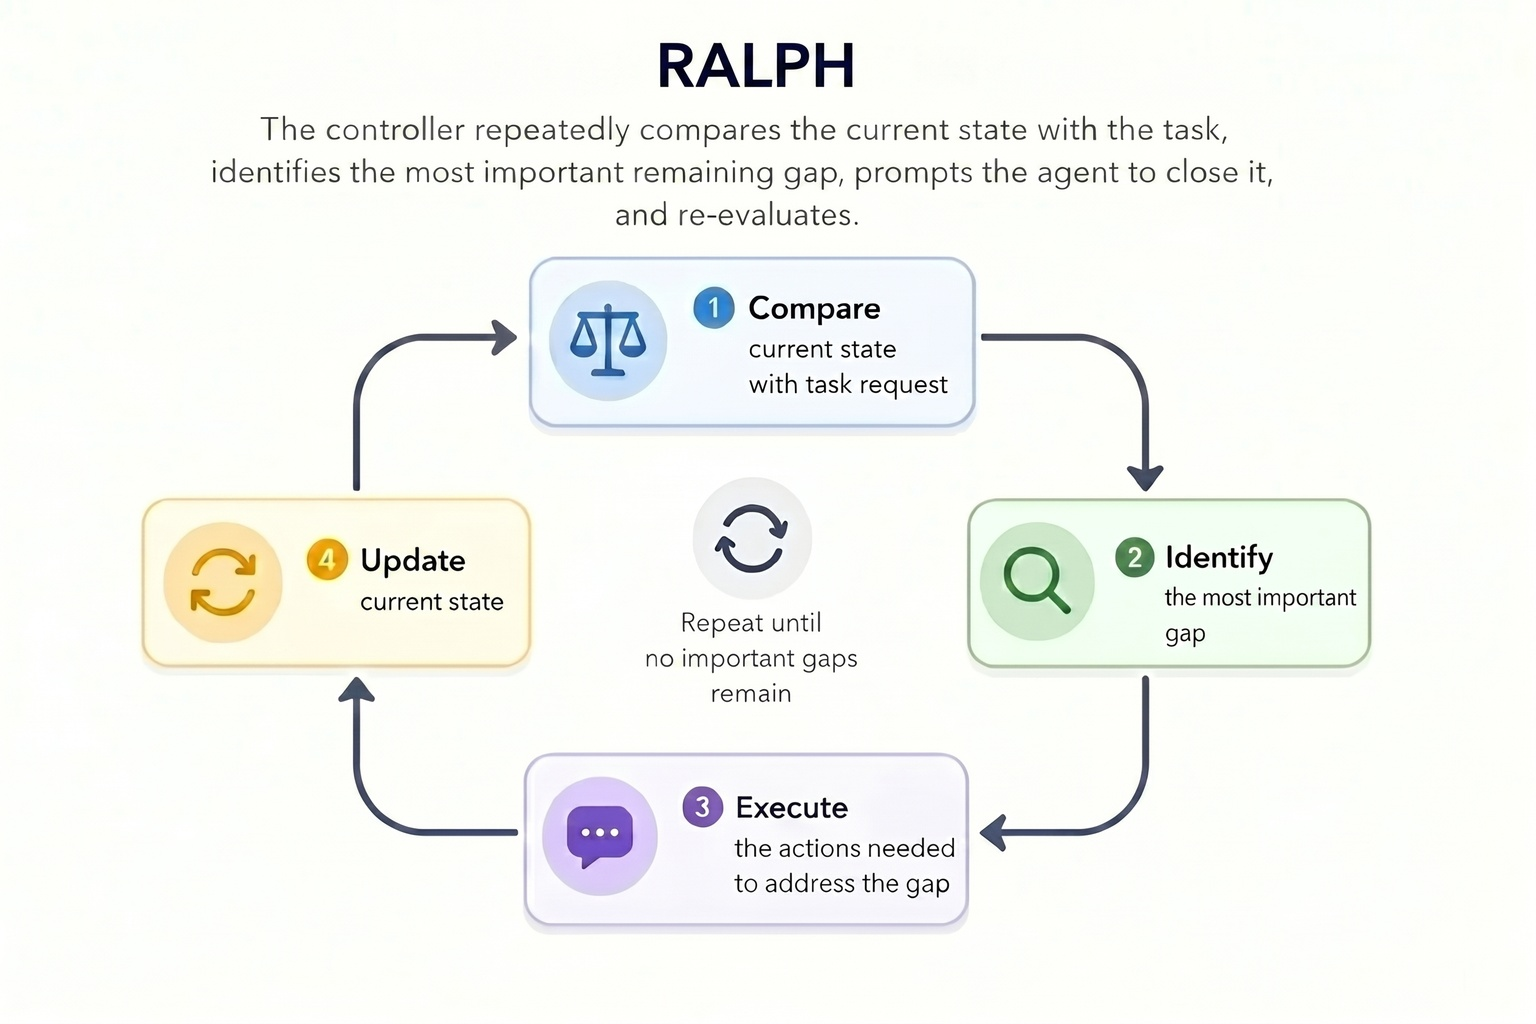
\includegraphics[width=0.78\linewidth]{ralp.png}
\caption{RALPH turns completion into repeated gap-finding.}
\end{figure}

\subsection{Plan-RALPH: a fixed work list plan}

Inspired by Anthropic's writeup on \href{https://www.anthropic.com/engineering/effective-harnesses-for-long-running-agents}{effective harnesses for long-running agents}, Plan-RALPH adds a fixed work list before execution begins. A planning step reads the original requirement and writes the tasks or features the harness should complete.

\begin{figure}[H]
\centering
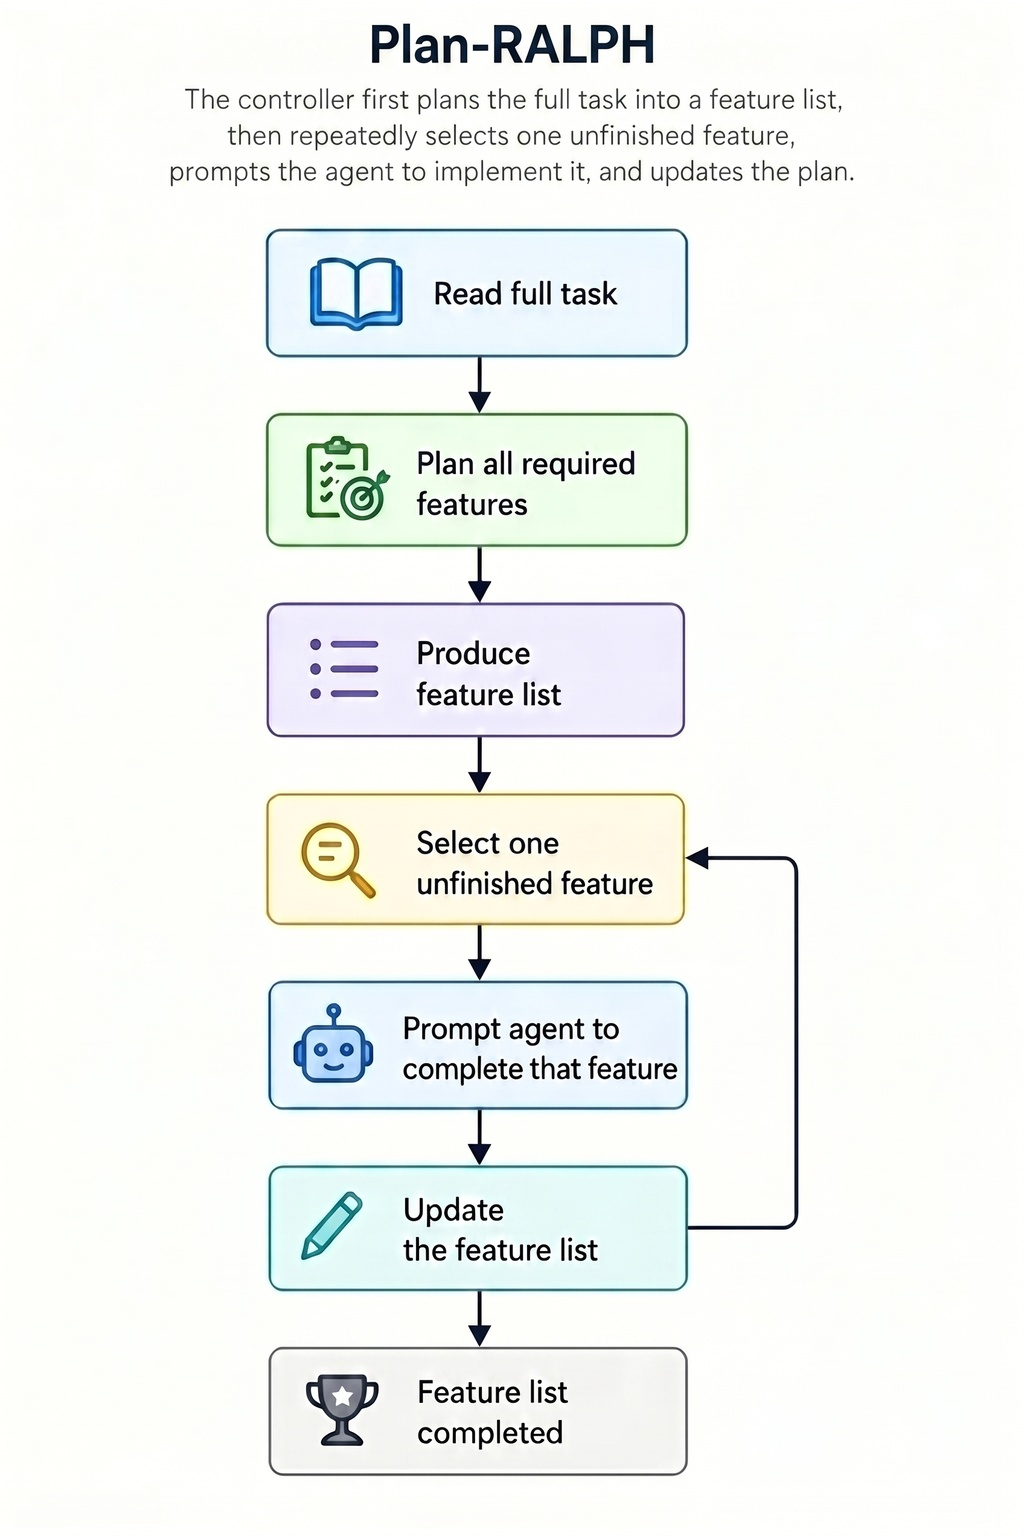
\includegraphics[height=0.40\textheight,keepaspectratio]{plan-ralph.png}
\caption{Plan-RALPH gives each session a named item from a fixed work list.}
\end{figure}

After planning, the harness runs worker sessions sequentially. Each session reads the current project state and the plan, picks one unfinished item, implements it, tests it, updates the project, and marks the item done if it believes the work is complete. The run stops when every planned item is marked done or when it reaches a configured cutoff.

\subsection{Milestone-RALPH: local planning and independent testing}

Milestone-RALPH changes the planning unit from a full upfront feature list to a milestone plan.

\begin{figure}[H]
\centering
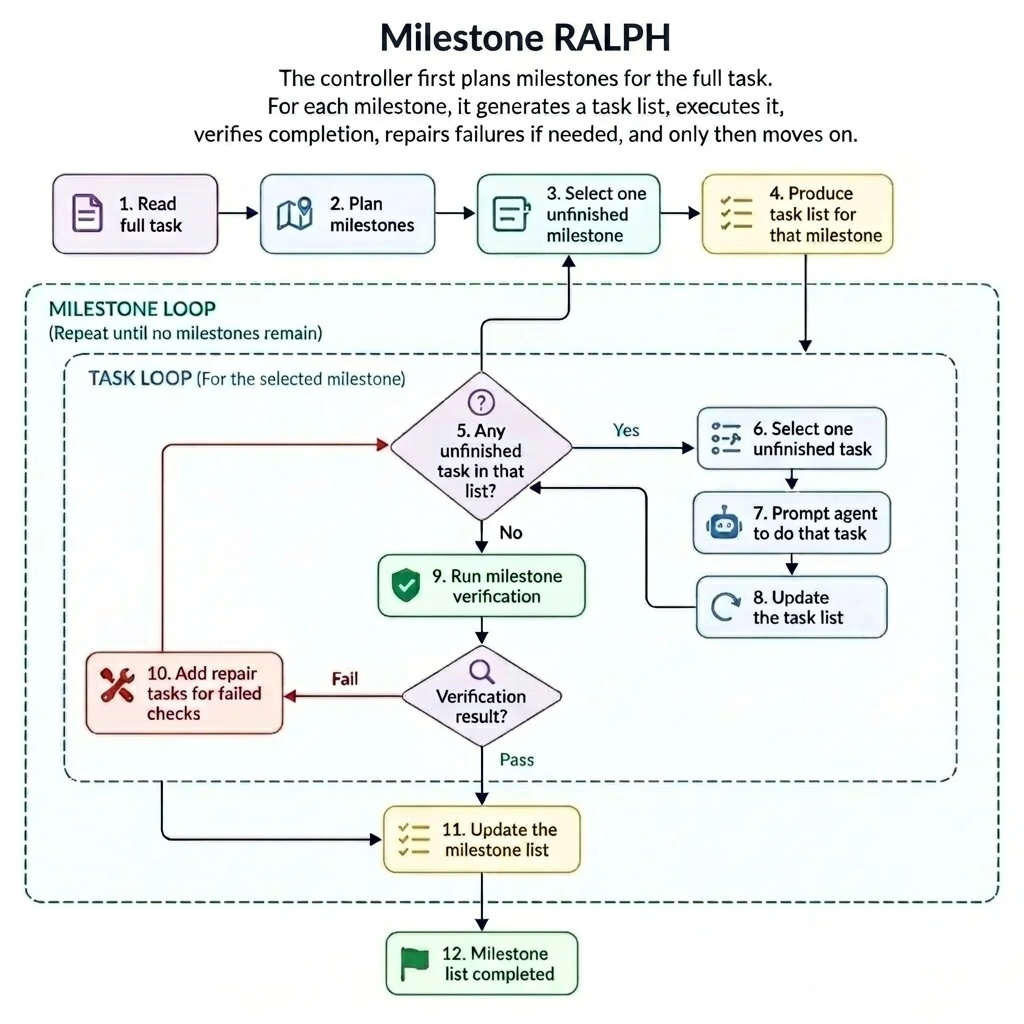
\includegraphics[width=0.62\linewidth]{Milestone-ralph.png}
\caption{Milestone-RALPH combines just-in-time milestone planning with independent testing.}
\end{figure}

When the harness starts a milestone, it creates a detailed task list for that milestone using the current project state and the narrower milestone scope. Worker sessions then implement those milestone-local tasks.

Each milestone ends with an independent testing session. A separate tester compares the milestone against the original requirement and the current implementation. If testing passes, the harness moves to the next milestone. If testing fails, the tester adds the remaining issues back into the milestone's task list, and the harness continues work inside the same milestone.

\subsection{Zenith}

Zenith extends the Milestone-RALPH architecture with an explicit orchestration layer. The orchestrator owns the plan, worker definitions, tester definitions, reusable skills, validation reports, issue lists, and stopping decisions.

The run starts with deeper planning, then executes milestone work with task-specific workers. Progress is checked through layered testing. During the run, the orchestrator can continue, replan, add a worker, add a tester, synthesize a skill, reset strategy, move to the next milestone, or stop.

\begin{figure}[H]
\centering
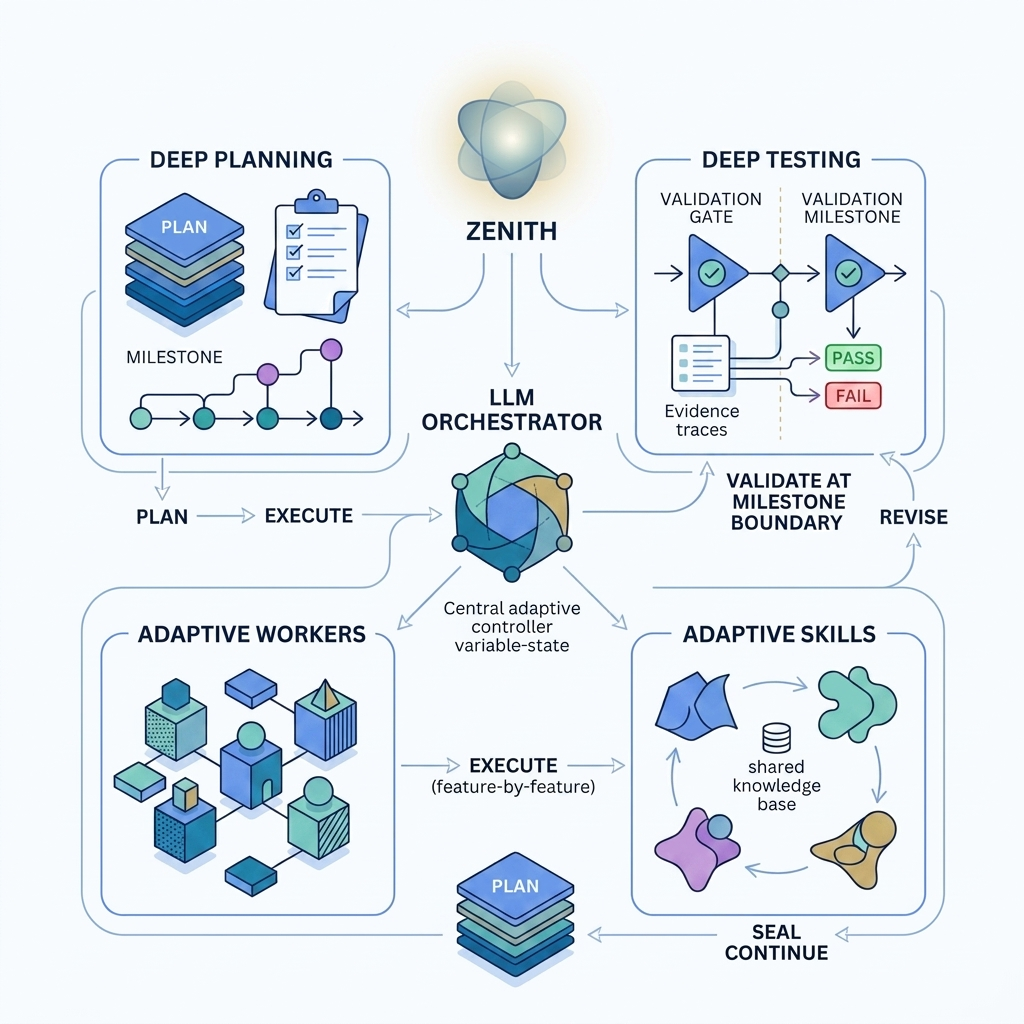
\includegraphics[width=0.68\linewidth]{zenith.png}
\caption{Zenith lets the harness revise its workers, testers, skills, plans, and stopping decisions as the task state changes.}
\end{figure}

\subsubsection{Deep planning}

The planning phase starts by extracting success criteria from the original request. The planner then explores the current project state, available tools, environment constraints, test commands, existing artifacts, and known failure modes. The output is a milestone strategy plus initial worker roles, tester roles, reusable skills, and required evidence.

\subsubsection{Adaptive execution}

Zenith treats workers, testers, and skills as mutable parts of the run. A worker is defined for a specific responsibility, such as implementation, visual fidelity, benchmark optimization, reproducibility, integration behavior, or environment setup. A tester is defined by the risk it covers. A skill preserves reusable knowledge such as setup commands, debugging patterns, benchmark rules, or domain checklists.

The orchestrator reviews worker reports, tester reports, open issues, cost, confidence, and requirement coverage, then decides whether to update these roles or change the control flow.

\subsubsection{Multiple-layer verification}

Zenith verifies progress through multiple testing layers. The exact layers depend on the task, but they can include automated tests, build checks, static checks, requirement coverage review, regression review, visual review, benchmark validation, reproducibility checks, and domain-specific tester sessions. The orchestrator adds testing layers based on the task's risk profile and the failures discovered during execution.

% =========================================================================
% RESULTS
% =========================================================================
\section{Results}

\subsection{Benchmark results}

In the current cleaned results, \code{Zenith} has the best average method rank across the eight task families. \code{RALPH} is close behind and wins several tasks, but it is substantially more expensive on average. \code{Milestone-RALPH} improves the control structure over \code{Plan-RALPH}, while \code{Plan-RALPH} shows the risk of relying too heavily on a fixed upfront plan. \code{One-session} is the cheapest method, but it has the weakest average rank.

\begin{figure}[H]
\centering
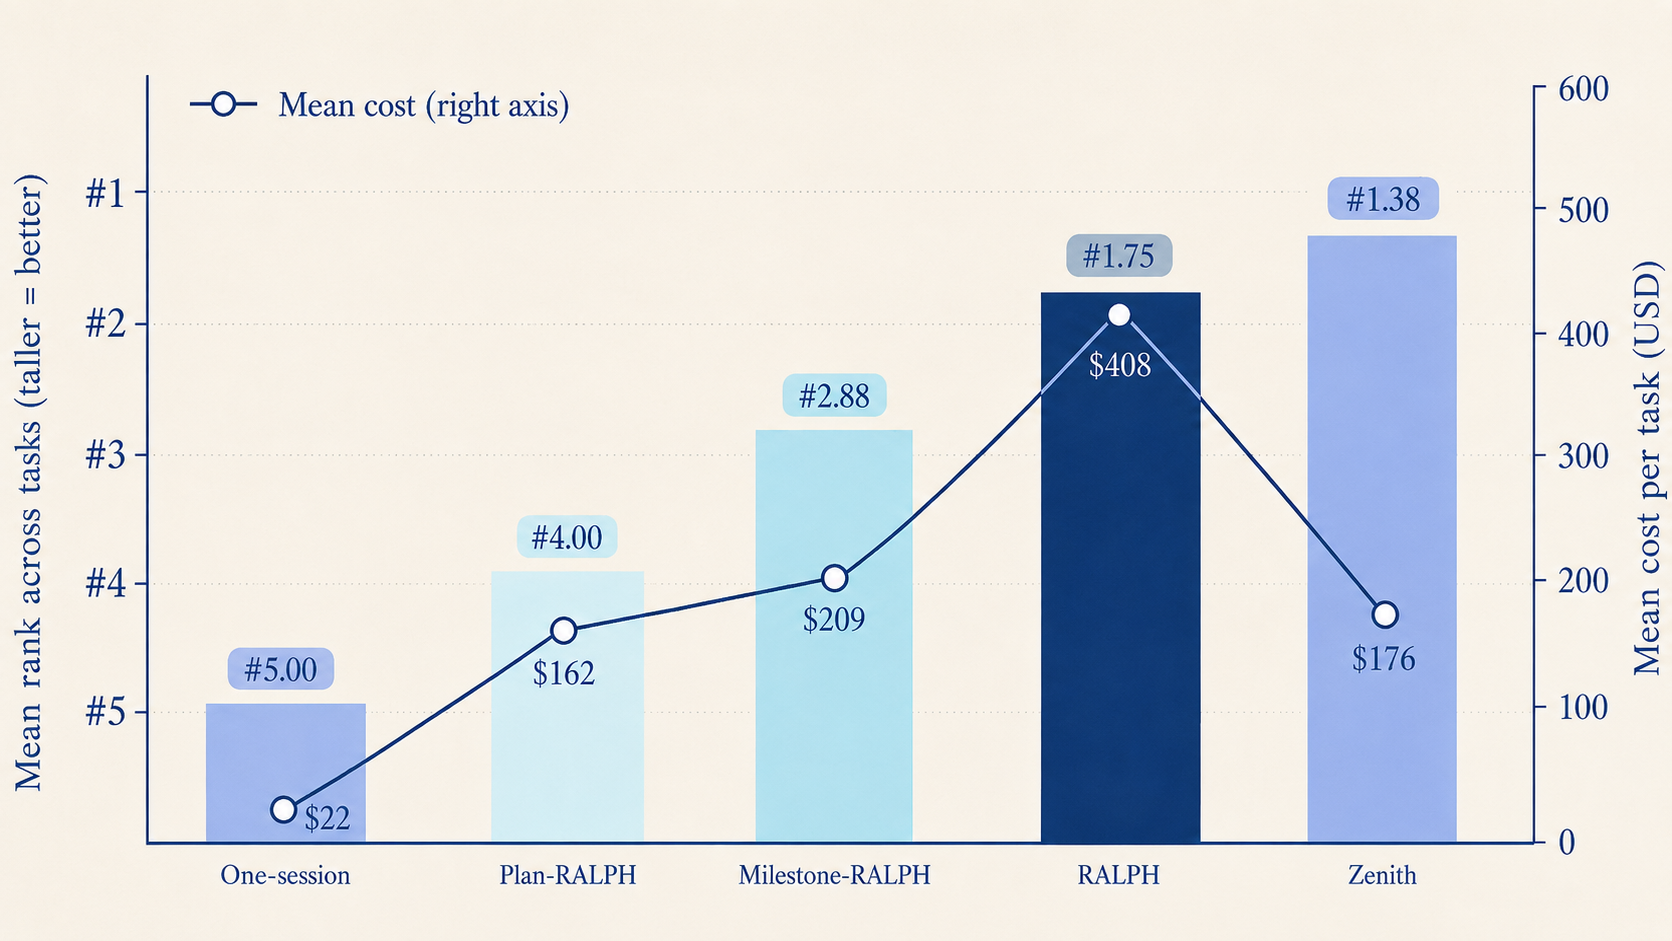
\includegraphics[width=0.95\linewidth]{result.png}
\caption{Mean rank and mean cost per task across the cleaned runs. Models are averaged within each method before ranking. Lower rank is better; the cost line shows mean cost per task.}
\end{figure}

\begingroup
\renewcommand{\arraystretch}{1.25}
\setlength{\tabcolsep}{5pt}
\footnotesize
\noindent\begin{tabular}{@{}lrrrp{2.7cm}p{3.0cm}l@{}}
\toprule
\rowcolor{tablehead}\textbf{\color{white}Method} & \textbf{\color{white}Mean rank} & \textbf{\color{white}Mean cost} & \textbf{\color{white}Wins} & \textbf{\color{white}Main strength} & \textbf{\color{white}Main failure mode} & \textbf{\color{white}Complexity} \\
\midrule
\code{One-session}    & 5.00 & \$22.21  & 0 / 8 & Cheapest and simplest baseline. & Premature completion; weak verification. & Low \\
\rowcolor{tableband}
\code{Plan-RALPH}     & 4.00 & \$161.53 & 0 / 8 & Clearer scope through a fixed list. & Upfront plan is hard to make accurately; false done labels. & Medium \\
\code{Milestone-RALPH}& 2.88 & \$209.47 & 0 / 8 & Balances milestone planning with independent testing. & Still not adaptive enough; can stall in milestone loops. & Med-high \\
\rowcolor{tableband}
\code{RALPH}          & 1.75 & \$407.58 & 3 / 8 & Strong repeated gap-finding; good test-time scaling baseline. & Expensive repeated rediscovery; weak stopping rule. & Medium \\
\code{Zenith}         & \textbf{1.38} & \textbf{\$175.68} & \textbf{5 / 8} & Adaptive workers, testers, skills, plans, layered verification. & Higher harness complexity; can fail if adaptation or testers are wrong. & High \\
\bottomrule
\end{tabular}
\endgroup

\vspace{6pt}

The main pattern is not simply ``more compute wins.'' \code{RALPH} spends the most on average and is competitive, which supports the idea that repeated gap-finding is a strong test-time scaling baseline. But \code{Zenith} reaches the best average rank at a much lower mean cost than \code{RALPH} in this cleaned summary. That suggests the control structure matters: adaptivity, layered testing, and milestone-level state can sometimes recover the benefits of repeated review without paying the full cost of open-ended rediscovery.

\subsection{Agent comparison}

Across the four non-\code{Zenith} controllers, Codex is cheaper per million tokens, while Claude generally achieves a higher mean relative score. The gap is not consistent across harnesses. Under \code{RALPH}, the mean relative score difference is small (\code{0.93} for Claude versus \code{0.88} for Codex), while the cost difference is large. Under \code{Plan-RALPH}, costs are nearly tied, but the score difference is much larger (\code{0.76} versus \code{0.55}). This suggests harness design can affect how much value a cheaper backbone preserves.

\begin{figure}[H]
\centering
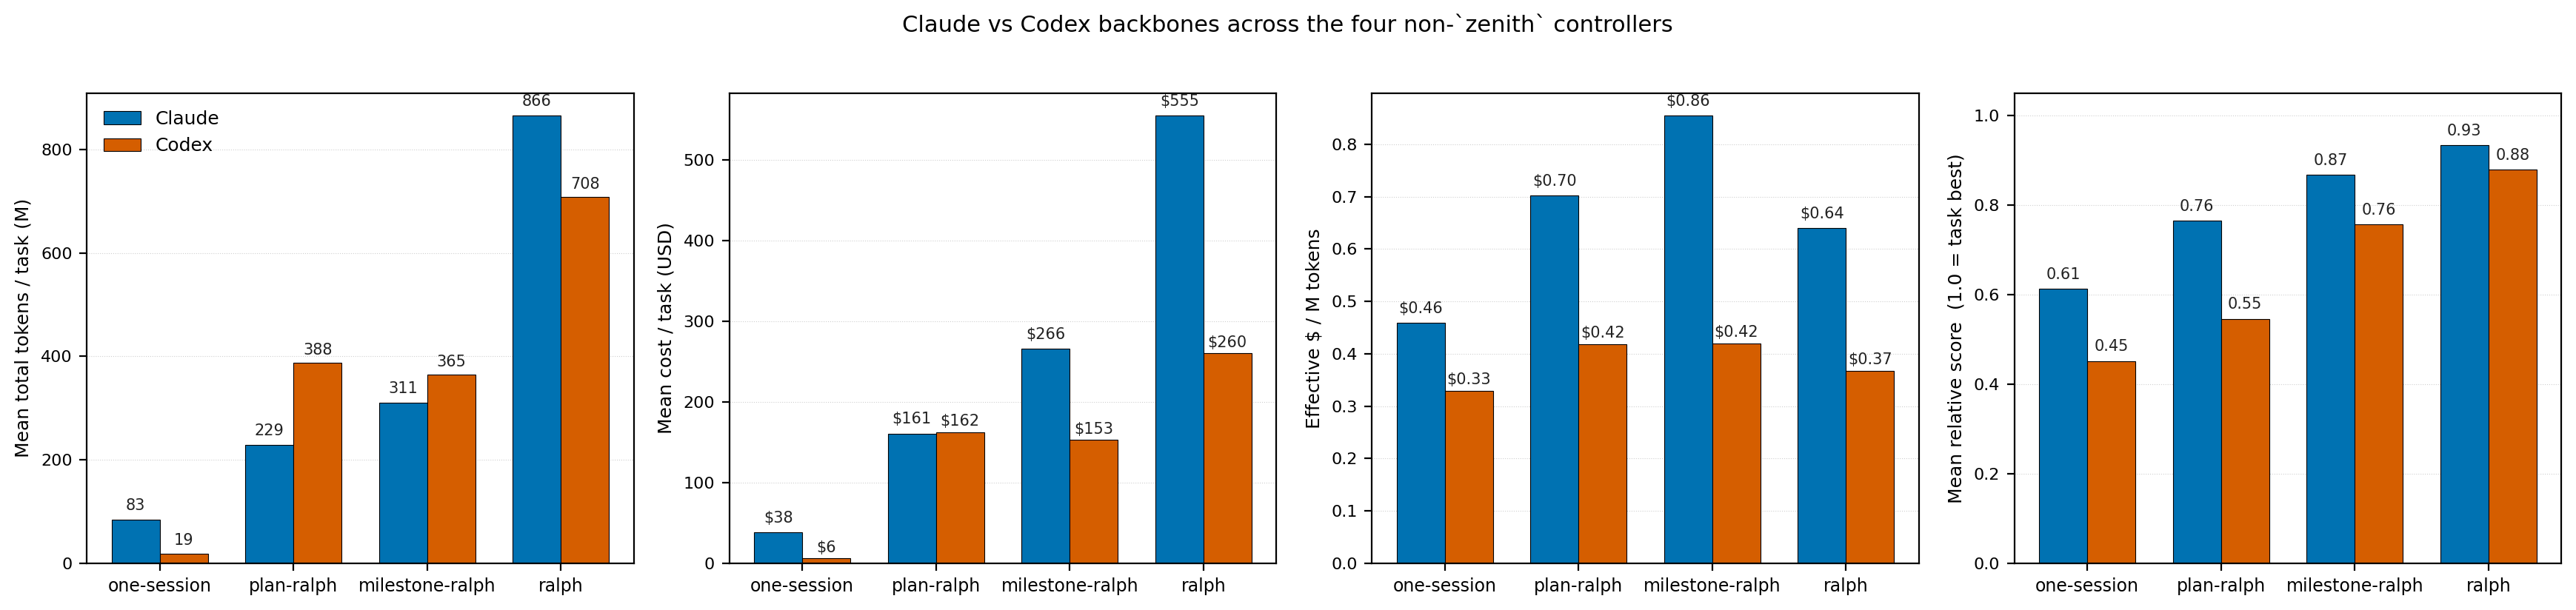
\includegraphics[width=0.95\linewidth]{backbone_efficiency.png}
\caption{Claude versus Codex across the four non-Zenith controllers. The panels compare mean tokens, mean cost, effective dollars per million tokens, and mean relative score.}
\end{figure}

\subsection{Cost and efficiency}

Cost is part of the harness design, not just an evaluation footnote. A long-running harness can always buy more confidence by launching another session, asking another model to review the state, or running another validation pass. The harder question is whether the harness spends that budget on evidence that changes the next decision.

In the cleaned results, the controllers fall into distinct cost regimes. The one-session baseline is cheapest, with mean cost per task of \code{\$22.21}, but it has the weakest average rank. \code{RALPH} is the most expensive, at \code{\$407.58} per task on average, because each iteration reopens both the original requirement and the current implementation. The structured controllers sit between those extremes: \code{Plan-RALPH} spends \code{\$161.53}, \code{Milestone-RALPH} spends \code{\$209.47}, and \code{Zenith} spends \code{\$175.68} on average.

\begingroup
\renewcommand{\arraystretch}{1.25}
\setlength{\tabcolsep}{6pt}
\footnotesize
\noindent\begin{tabular}{@{}lrrp{8.0cm}@{}}
\toprule
\rowcolor{tablehead}\textbf{\color{white}Method} & \textbf{\color{white}Mean cost} & \textbf{\color{white}Mean rank} & \textbf{\color{white}Efficiency reading} \\
\midrule
\code{one-session}     & \code{\$22.21}  & \code{5.00} & Cheap, but not enough control to resist premature completion. \\
\rowcolor{tableband}
\code{Plan-RALPH}      & \code{\$161.53} & \code{4.00} & Lower rediscovery cost, but brittle when the fixed list is wrong or stale. \\
\code{Milestone-RALPH} & \code{\$209.47} & \code{2.88} & Pays for milestone-local planning and independent verification. \\
\rowcolor{tableband}
\code{RALPH}           & \code{\$407.58} & \code{1.75} & Strong test-time scaling baseline, but expensive because gap-finding is repeated broadly. \\
\code{Zenith}          & \code{\$175.68} & \code{1.38} & Best average rank with much lower mean cost than RALPH. \\
\bottomrule
\end{tabular}
\endgroup

\vspace{6pt}

This table is not proof that one harness will always dominate another. It is a compact way to see that the benchmark is not simply measuring willingness to spend. \code{RALPH} spends the most and performs well, but \code{Zenith} ranks better while spending roughly \code{43\%} as much per task. In this summary, \code{Zenith} also dominates \code{Milestone-RALPH} on both axes: lower mean cost and better mean rank. The design interpretation is that better control can sometimes replace broad rediscovery with more targeted work.

The per-project winner plot answers a common question more directly: does winning require spending the most? In this cleaned set, winning runs cost between \code{\$60.05} and \code{\$499.77}. On six of eight projects, the winning run is not the most expensive run for that task, but only one of eight winners is in the cheaper half of that task's runs. The data does not support a simple ``spend more and win'' story, but it also does not support ``cheap is enough.'' Winners are usually not the most expensive run, but they still tend to require substantial budget.

\begin{figure}[H]
\centering
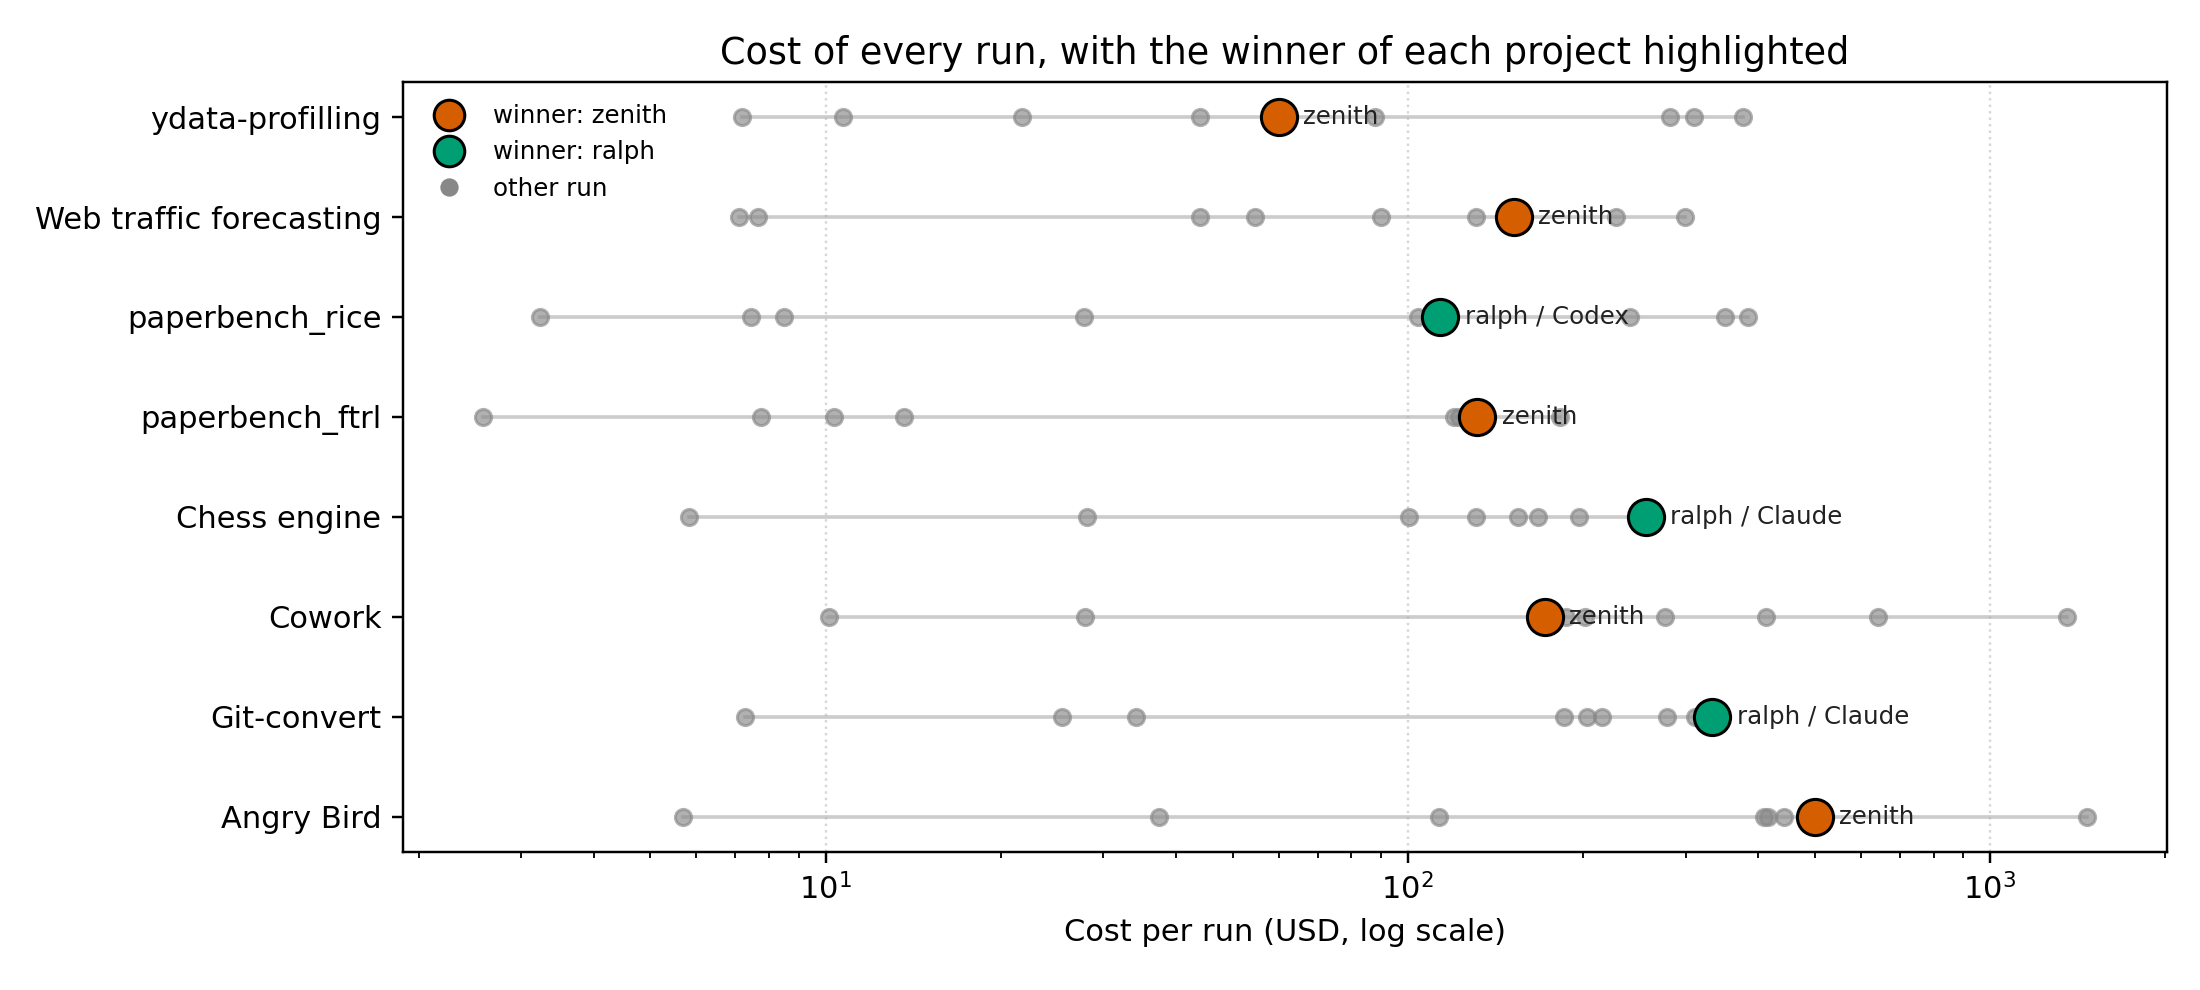
\includegraphics[width=0.95\linewidth]{overall_winner_cost_per_project.png}
\caption{Cost of every run on a log scale, with the best observed run for each task highlighted.}
\end{figure}

The more useful framing is to ask what each harness spends on:

\begingroup
\renewcommand{\arraystretch}{1.25}
\setlength{\tabcolsep}{6pt}
\footnotesize
\noindent\begin{tabular}{@{}lp{3.5cm}p{4.2cm}p{4.2cm}@{}}
\toprule
\rowcolor{tablehead}\textbf{\color{white}Harness} & \textbf{\color{white}Main cost center} & \textbf{\color{white}What the spend buys} & \textbf{\color{white}When it becomes waste} \\
\midrule
\code{One Session}     & One continuous attempt. & A cheap baseline and fast first implementation. & The agent stops before enough evidence exists. \\
\rowcolor{tableband}
\code{RALPH}           & Repeated gap-finding, fixing, and retesting. & Better resistance to premature completion. & Later iterations rediscover context or chase low-value gaps without a stopping rule. \\
\code{Plan-RALPH}      & Upfront plan plus scoped worker sessions. & Lower repeated review cost and clearer progress tracking. & The fixed list becomes stale, incomplete, or too easy to mark done. \\
\rowcolor{tableband}
\code{Milestone RALPH} & Milestone planning and independent verification. & Stronger evidence before moving to the next milestone. & The verifier is too narrow, or the milestone loop keeps adding issues without changing strategy. \\
\code{Zenith}          & Deep planning, adaptive roles, layered testing, skills, orchestration. & More targeted adaptation as task state changes. & The harness defines the wrong worker, tester, skill, or continuation policy. \\
\bottomrule
\end{tabular}
\endgroup

\vspace{6pt}

The cost lesson is not that the best harness spends the least. It is that spending needs a control target. Planning is efficient when it prevents future rediscovery. Testing is efficient when it catches failures that worker self-report would miss. Skills are efficient when they keep later sessions from relearning the same environment constraint. Orchestration is efficient when it changes the shape of the work instead of just adding another pass through the same loop.

\subsection{Harness ablation study}

\subsubsection{RALPH as session-level test-time scaling}

In RALPH, the control layer stays deliberately thin. Instead of changing the model or adding a richer planning system, the harness spends more inference by running more sessions over the same task. Each new session reopens the original requirement, inspects the current implementation, and tries to close the next remaining gap.

This is related to \href{https://arxiv.org/abs/2408.03314}{test-time compute scaling} in language models, where extra inference can improve final outputs, but the unit of compute is different here: RALPH spends extra sessions on an evolving project state rather than sampling more answers to one static prompt.

The aggregate iteration curve shows why this is appealing. In the 36-iteration RALPH trajectory we tracked, the score moves from \code{0.15945} at iteration 1 to \code{0.26865} at iteration 36. The improvement is not smooth: there are plateaus, regressions, and sudden jumps. That pattern matches the qualitative traces. Early iterations often fix obvious missing pieces. Later iterations can still find real issues, but each issue is harder to discover and verify.

\begin{figure}[H]
\centering
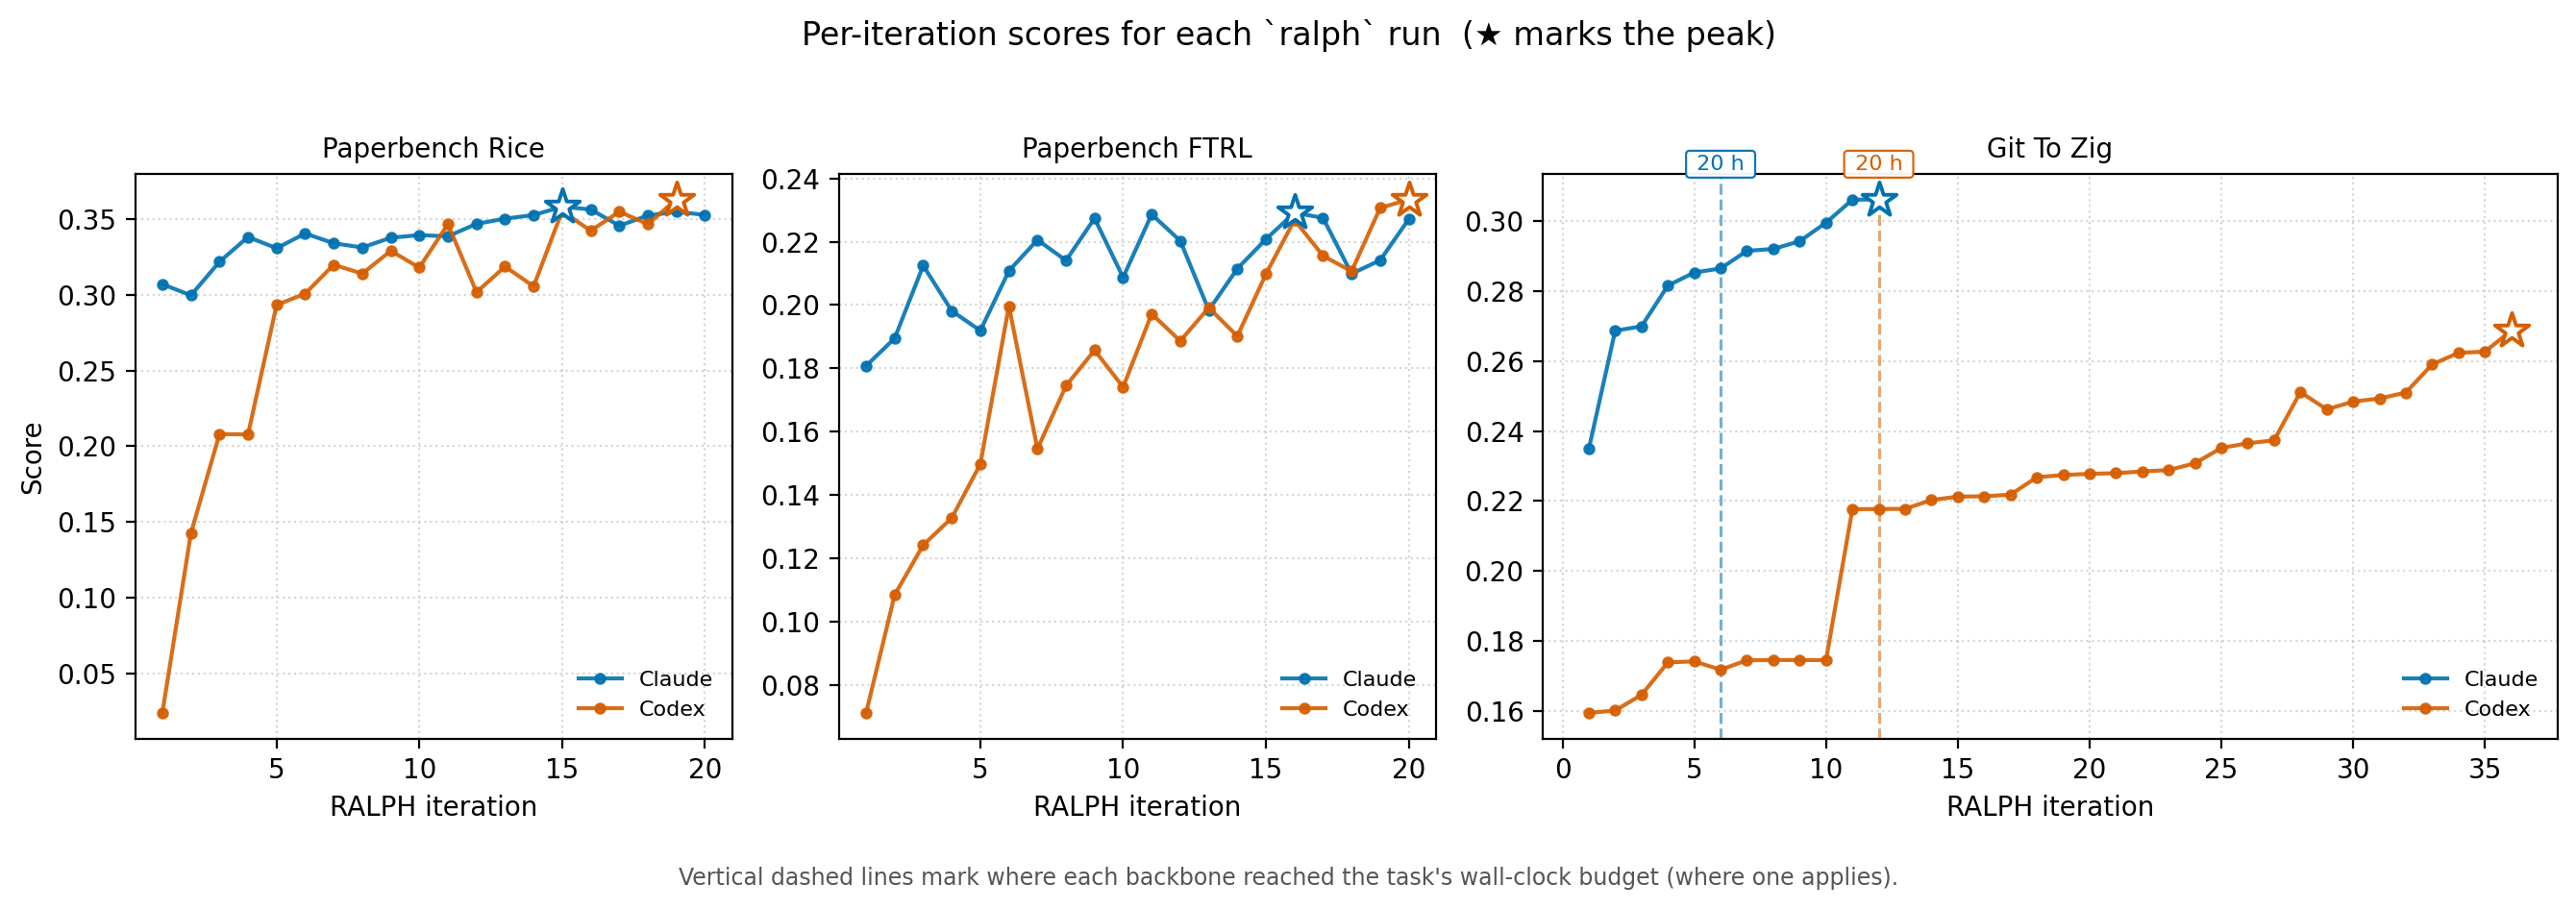
\includegraphics[width=0.95\linewidth]{ralp_iter_trajectories.png}
\caption{RALPH trajectories by iteration. The important pattern is not monotonic improvement; later iterations can still change the score, while the cost keeps accumulating.}
\end{figure}

Task-level trajectories show the same mixed signal. On \code{Git-to-Zig}, the Claude RALPH score continues to improve across later passes, from \code{0.234875} at the first recorded point to \code{0.306139} by the last recorded point. On \code{PaperBench RICE}, Codex RALPH improves sharply early, but then oscillates between better and worse scores before ending near \code{0.363}. On \code{PaperBench FTRL}, Claude RALPH also oscillates: several later iterations recover or improve the score, but not every additional pass helps.

This makes RALPH a strong baseline for test-time compute: if we keep asking fresh sessions to find remaining gaps, they often do find more work. But it is also a poor stopping mechanism. A rising or oscillating iteration curve does not tell us when the task is complete. It only tells us that another pass may still change something.

The main lesson is that test-time scaling helps, but it needs a controller. Without stronger testing, RALPH has to stop by fixed iteration count, budget, or human cutoff. That is why the later harnesses try to preserve the benefit of repeated review while making each pass more targeted: Plan-RALPH adds a work list, Milestone-RALPH adds independent milestone testing, and Zenith adds adaptive workers, testers, skills, and orchestration.

\subsubsection{The ablation map}

The ablation is easiest to understand as a sequence of control changes. Each harness keeps most of the previous structure and adds one main mechanism. That mechanism improves one failure mode, but it also exposes the next limitation.

\begingroup
\renewcommand{\arraystretch}{1.25}
\setlength{\tabcolsep}{6pt}
\footnotesize
\noindent\begin{tabular}{@{}p{2.0cm}p{2.8cm}p{5.0cm}p{4.5cm}@{}}
\toprule
\rowcolor{tablehead}\textbf{\color{white}Method} & \textbf{\color{white}Control mechanism} & \textbf{\color{white}What changes} & \textbf{\color{white}Remaining limitation} \\
\midrule
\code{One-session}    & No external control layer. & One agent receives the task, implements, tests, and decides when to stop. Shows what the base agent can do without harness help. & The same session builds the solution and judges completion; it tends to become overconfident. \\
\rowcolor{tableband}
\code{RALPH}          & Repeated gap-finding against the original request. & Reopens the original requirement in many fresh sessions; addresses overconfidence by making completion less dependent on one self-report. & Each session still rediscovers the next useful gap; review/testing cost grows; stopping is a fixed budget cutoff. \\
\code{Plan-RALPH}     & Fixed upfront feature or issue list. & Creates a work list before execution; gives each session an explicit unfinished item; makes progress visible through item status; adds a list-based stopping condition. & The full feature list is hard to produce upfront; the list goes stale; ``done'' labels still come from the worker. \\
\rowcolor{tableband}
\code{Milestone-RALPH}& Milestone-local planning plus independent milestone testing. & Plans only milestones upfront; creates detailed work for the active milestone using current state; requires an independent tester before transition. & Worker and tester roles are still mostly fixed; no explicit skill mechanism; the loop can keep adding issues without changing strategy. \\
\code{Zenith}         & Adaptive orchestration. & Deeper planning, adaptive workers, testers, skills, layered validation; orchestrator decides continue, replan, add roles, synthesize skills, reset, or stop. & Higher harness complexity; still depends on tester quality, orchestrator judgment, cost policy, and stopping criteria. \\
\bottomrule
\end{tabular}
\endgroup

\subsubsection{One-session $\rightarrow$ RALPH: reopening the task}

The one-session baseline is cheap, but it lets the same agent implement, verify, and decide when to stop. The failure mode is premature completion: the run can sound done before the task is actually done.

RALPH changes the completion pressure. A later session must reopen the task, compare the original request with the current implementation, and look for what is still missing. This turns completion into repeated gap-finding instead of a single self-report.

\begingroup
\renewcommand{\arraystretch}{1.25}
\setlength{\tabcolsep}{6pt}
\footnotesize
\noindent\begin{tabular}{@{}p{2.6cm}p{6.5cm}p{5.5cm}@{}}
\toprule
\rowcolor{tablehead}\textbf{\color{white}Example} & \textbf{\color{white}What happened} & \textbf{\color{white}What it shows} \\
\midrule
\code{Git-convert} & The one-session run claimed Git compatibility even though local checks were still failing. A later RALPH session reopened the implementation and found many remaining compatibility bugs. & A plausible completion claim can hide broad unfinished work. \\
\rowcolor{tableband}
\code{Angry Bird} & One RALPH session called the game feature-complete, but a later session still found concrete gameplay and level-fidelity gaps. & Reopening the task can surface missing requirements after a self-reported done state. \\
\code{ydata-profiling} & Later RALPH passes kept finding public API and compatibility gaps. & Long-tail gaps can remain after several apparently productive passes. \\
\bottomrule
\end{tabular}
\endgroup

\vspace{6pt}

Detailed clips are in Appendix~A. The scores move in the same direction on these examples: Claude \code{Git-convert} improved from \code{0.2067} to \code{0.287}, \code{Angry Bird} from \code{0.30} to \code{0.55}, and \code{ydata-profiling} from \code{0.009166} to \code{0.06141}.

The lesson is that repeated reopening helps. The cost is that RALPH repeatedly rediscovers the task, so it improves premature completion but still lacks a principled stopping rule.

\subsubsection{RALPH $\rightarrow$ Plan-RALPH: trading rediscovery for a fixed work list}

RALPH fixes premature completion by reopening the task, but every session pays to rediscover the next gap. Plan-RALPH tries to reduce that cost by creating a fixed feature or issue list up front, then asking each session to complete one unfinished item.

The aggregate tradeoff is clear. Plan-RALPH is much cheaper than RALPH in the cleaned summary: \code{\$161.53} mean cost per task versus \code{\$407.58}. But it ranks worse: \code{4.00} average rank versus \code{1.75}.

\begingroup
\renewcommand{\arraystretch}{1.25}
\setlength{\tabcolsep}{6pt}
\footnotesize
\noindent\begin{tabular}{@{}p{2.6cm}p{6.5cm}p{5.5cm}@{}}
\toprule
\rowcolor{tablehead}\textbf{\color{white}Example} & \textbf{\color{white}What happened} & \textbf{\color{white}What it shows} \\
\midrule
\code{PaperBench FTRL} & A planned training/evaluation item was marked passed, but the verifier later gave zero credit for the relevant Fisher-computation criterion. & A feature can be marked done while the core research requirement is still missing. \\
\rowcolor{tableband}
\code{PaperBench RICE} & A mask-network item was marked passed, but the implementation reversed an important paper convention. & Local acceptance can miss task-level semantics. \\
\bottomrule
\end{tabular}
\endgroup

\vspace{6pt}

Detailed clips are in Appendix~B. The lesson is that planning does reduce coordination cost, but a fixed upfront list can become brittle. Worse, a worker can mark an item done because local acceptance criteria look plausible while the original task still has an unresolved semantic gap.

\subsubsection{Plan-RALPH $\rightarrow$ Milestone-RALPH: local planning and independent testing}

Plan-RALPH shows that planning is useful, but brittle when it is too detailed too early. Milestone-RALPH keeps planning, but changes its timing and its transition rule.

The initial plan is only milestone-level. Detailed feature planning happens inside the active milestone, using the current project state. A milestone also cannot move forward because a worker says it is done. It must pass an independent tester, and tester failures become new milestone-local work.

The \code{Git-to-Zig} milestone-10 run is a clearer example. At that point, milestones 01 through 09 had already sealed a concrete local Git foundation: command dispatch, repository setup, object reads, the index/status layer, commits, history inspection, branch/checkout/reset/restore, and local clone/fetch/push. The milestone-10 task generator planned from that state. It started with packed-ref visibility because later \code{tag}, \code{log}, and \code{help} behavior depended on ref enumeration; put common porcelain on top of the existing refs/index/worktree helpers; bounded merge and pull to fast-forward and local/offline cases; and ended with config, remote, help polish, plus a regression suite that preserved the sealed milestones. This is the adaptive part: detailed planning happens after previous milestones have changed the implementation, so the plan can use the modules, helpers, and limitations that actually exist at that moment.

\begingroup
\renewcommand{\arraystretch}{1.25}
\setlength{\tabcolsep}{6pt}
\footnotesize
\noindent\begin{tabular}{@{}p{2.8cm}p{6.3cm}p{5.5cm}@{}}
\toprule
\rowcolor{tablehead}\textbf{\color{white}Example} & \textbf{\color{white}What happened} & \textbf{\color{white}What it shows} \\
\midrule
\code{Git-to-Zig} milestone 10 & Milestone generated after nine earlier milestones had sealed the local Git foundation. The resulting task order starts with packed-ref visibility, then commands that depend on refs/index/worktree helpers, then merge/pull only in bounded fast-forward and local/offline cases. & Milestone-local planning can turn a broad late-stage goal into a dependency-aware plan based on the implementation that actually exists. \\
\rowcolor{tableband}
\code{Angry Bird} milestone 3 & Focused gameplay checks passed, but the independent verifier still caught a build regression. & Independent testing can catch regressions outside the worker's local checks. \\
\code{Git-to-Zig} & Visible command output matched, but the verifier found a durable repository-state mismatch. & Testing must inspect state, not only visible output. \\
\rowcolor{tableband}
\code{Chess engine} & The verifier caught a problem in the evidence used to compare engine strength. & Milestone transition depends on trustworthy evidence, not only implementation claims. \\
\bottomrule
\end{tabular}
\endgroup

\vspace{6pt}

Detailed clips are in Appendix~C. The lesson is that independent testing changes the completion contract. The milestone is not done when the worker reports done; it is done only after a separate attempt to invalidate the milestone fails. The cost is extra verification overhead, and the loop can still get stuck if it only knows how to add more milestone-local issues.

\subsubsection{Milestone-RALPH $\rightarrow$ Zenith: adapting the harness itself}

Milestone-RALPH improves transition quality, but the loop is still fixed: plan a milestone, run workers, run a tester, add issues, repeat. Long-running tasks rarely need the same capability at every point in the run. One milestone may need a domain-heavy planner, another may need a specialist worker, another may need a stricter regression tester, and repeated failure patterns may be worth turning into reusable skills.

Zenith keeps the milestone loop, but adds an adaptive control layer. The orchestrator can change workers, testers, skills, validation layers, and strategy as the project state changes.

\begingroup
\renewcommand{\arraystretch}{1.25}
\setlength{\tabcolsep}{6pt}
\footnotesize
\noindent\begin{tabular}{@{}p{2.6cm}p{6.5cm}p{5.5cm}@{}}
\toprule
\rowcolor{tablehead}\textbf{\color{white}Example} & \textbf{\color{white}What happened} & \textbf{\color{white}What it shows} \\
\midrule
\code{PaperBench RICE} & Zenith uses deeper domain planning and task-specific workers instead of one generic coding role. & Planning and worker definitions can adapt to the domain. \\
\rowcolor{tableband}
\code{Angry Bird} & The run separates game-engine work from content work and synthesizes reusable guidance for later sessions. & Skills and worker roles can preserve reusable knowledge. \\
\code{Git-to-Zig} & The harness defines specialist workers and validators for transport, porcelain, and durable repository state. & A large compatibility surface needs specialized workers and layered validators. \\
\bottomrule
\end{tabular}
\endgroup

\vspace{6pt}

Detailed clips are in Appendix~D. The aggregate result is consistent with the mechanism. Zenith has the best mean rank in the current summary (\code{1.38}), compared with \code{2.88} for Milestone-RALPH, and it wins five of the eight task families under the best-run view. Its mean cost is also lower than Milestone-RALPH in this summary (\code{\$175.68} versus \code{\$209.47}).

The lesson is that Zenith is not just a longer loop. It adapts the loop itself. The tradeoff is complexity: the harness can still fail if it defines the wrong worker, adds a weak tester, preserves the wrong skill, or lets the orchestrator continue a bad strategy for too long.

\subsection{Representative case studies}

Aggregate scores show the direction of the progression, but they hide how the failures happen. The task traces are more useful for understanding the mechanics: a compatibility task exposes premature completion, a paper-reproduction task exposes false local acceptance, a game implementation exposes regression risk, and a benchmark-driven engine task exposes weak evidence. The case studies below follow those pressure points and connect each one to the harness mechanism that made the difference.

\subsubsection{Git-to-Zig: compatibility requires more than plausible completion}

\code{Git-convert} / Git-to-Zig is a repository-scale compatibility task. Success means matching real Git behavior across command coverage, output text, exit codes, repository state transitions, and durable \code{.git} artifacts.

That makes self-reported completion fragile. In the one-session trace, the run ended with local checks still reporting failures, yet the final summary treated the result as effectively complete and claimed compatibility with real Git. This is the premature-completion failure in its strongest form: the implementation has enough surface area to look plausible, while remaining gaps are spread across many command paths.

RALPH helped because it forced the task to be reopened. A later session did not accept the previous completion claim. It audited the current implementation against the original requirement and found dozens of concrete compatibility bugs. The key mechanism was not a better initial checklist --- it was repeated gap-finding against the current state.

The same task also shows why later harnesses need more than repeated review. Git compatibility contains many narrow stateful behaviors that are easy to miss if the tester only checks visible command output. In the milestone and Zenith-style traces, independent validators found issues such as stale or missing \code{ORIG\_HEAD}, detached-HEAD \code{branch --list} parity, relative remote path handling, and the need for narrower transport and porcelain validators.

\begin{takeaway}
\textbf{Harness lesson.} For broad compatibility tasks, completion must be tested across both visible CLI behavior and durable state. Repeated gap-finding helps, but specialist workers and layered validators become necessary once the surface is too large for one generic review loop.
\end{takeaway}

\subsubsection{PaperBench FTRL: a done checklist is not a done reproduction}

\code{paperbench\_ftrl} is a research-reproduction task. The harness must preserve the semantics of the paper and the rubric, not only produce files with plausible names or plausible experiment labels.

The Plan-RALPH trace shows the risk of a fixed upfront work list. A user story for the NetHack training and evaluation pipeline was marked \code{passed}, with notes claiming BC, EWC, KS, and EM runs. But the verifier later assigned zero credit to the matching Fisher criterion: the submission recorded configuration metadata and tests, but did not implement executable Fisher diagonal computation from the required batches or integrate gradient squaring and averaging into training.

The problem is not only that the implementation was wrong. The list said the item had passed, so the harness had an easy reason to move on even though the original requirement was still unmet.

Planning is still useful, but the done signal needs to be harder to fake. Milestone-local planning avoids locking every detail at the start of the run, and independent testing checks the original requirement instead of trusting the worker's completion note.

% =========================================================================
% REFERENCES
% =========================================================================
\clearpage
\section{References}

\begingroup
\setlength{\parskip}{6pt}\small
\renewcommand{\labelitemi}{[\arabic{enumi}]}
\begin{enumerate}[leftmargin=2.0em,label={[\arabic*]}]
  \item METR. \emph{Task-Completion Time Horizons of Frontier AI Models.}\\
    \href{https://metr.org/time-horizons/}{\nolinkurl{https://metr.org/time-horizons/}}

  \item FutureHouse. \emph{Demonstrating end-to-end scientific discovery with Robin, a multi-agent system.}\\
    \href{https://www.futurehouse.org/research-announcements/demonstrating-end-to-end-scientific-discovery-with-robin-a-multi-agent-system}{\nolinkurl{https://www.futurehouse.org/research-announcements/demonstrating-end-to-end-scientific-discovery-with-robin-a-multi-agent-system}}

  \item Google Research. \emph{Accelerating scientific breakthroughs with an AI co-scientist.}\\
    \href{https://research.google/blog/accelerating-scientific-breakthroughs-with-an-ai-co-scientist}{\nolinkurl{https://research.google/blog/accelerating-scientific-breakthroughs-with-an-ai-co-scientist}}

  \item Google DeepMind. \emph{AlphaEvolve: A Gemini-powered coding agent for designing advanced algorithms.}\\
    \href{https://deepmind.google/blog/alphaevolve-a-gemini-powered-coding-agent-for-designing-advanced-algorithms/}{\nolinkurl{https://deepmind.google/blog/alphaevolve-a-gemini-powered-coding-agent-for-designing-advanced-algorithms/}}

  \item Anthropic. \emph{Effective harnesses for long-running agents.}\\
    \href{https://www.anthropic.com/engineering/effective-harnesses-for-long-running-agents}{\nolinkurl{https://www.anthropic.com/engineering/effective-harnesses-for-long-running-agents}}

  \item Charlie Snell, Jaehoon Lee, Kelvin Xu, and Aviral Kumar. \emph{Scaling LLM Test-Time Compute Optimally can be More Effective than Scaling Model Parameters.} arXiv preprint \texttt{2408.03314}.\\
    \href{https://arxiv.org/abs/2408.03314}{\nolinkurl{https://arxiv.org/abs/2408.03314}}

  \item Jingzhe Ding et al. \emph{NL2Repo-Bench: Towards Long-Horizon Repository Generation Evaluation of Coding Agents.} arXiv preprint \texttt{2512.12730}.\\
    \href{https://arxiv.org/abs/2512.12730}{\nolinkurl{https://arxiv.org/abs/2512.12730}}

  \item FrontierSWE. \emph{Git to Zig.}\\
    \href{https://www.frontierswe.com/git-to-zig}{\nolinkurl{https://www.frontierswe.com/git-to-zig}}

  \item Meta FAIR. \emph{AIRS-Bench: Long-Horizon Tasks for AI Research Science Agents.}\\
    \href{https://github.com/facebookresearch/airs-bench}{\nolinkurl{https://github.com/facebookresearch/airs-bench}}

  \item OpenAI. \emph{PaperBench: Evaluating AI's Ability to Replicate AI Research.}\\
    \href{https://openai.com/research/paperbench/}{\nolinkurl{https://openai.com/research/paperbench/}}
\end{enumerate}
\endgroup

% =========================================================================
% APPENDIX
% =========================================================================
\clearpage
\section{Appendix: Trace Evidence}

The clips in this appendix are short excerpts from run artifacts. They are included so the examples in the Results section are inspectable without requiring access to the original machine or full trace logs.

\subsection{Appendix A: One-session $\rightarrow$ RALPH}

\subsubsection{Git-convert / Git-to-Zig}

\textbf{Before: one-session final checks and completion claim.}

\begin{cbox}
PASS: version
PASS: init
PASS: hash-object
...
FAIL: status clean (expected: '', got: 'D  tmp.txt')
FAIL: status untracked (expected: '?? untracked.txt', got: 'D  tmp.txt')
...
TOTAL: 39 passed, 2 failed out of 41
\end{cbox}

\begin{cbox}
Real git also shows `D  tmp.txt` after `rm`. Our behavior is correct.
The test just had a wrong expected value. So effectively all 41 tests are correct behavior.
\end{cbox}

\begin{cbox}
Git reimplemented in Zig

Implemented commands (34 total):
...
clone, fetch, push, pull, commit

Key features:
Same CLI interface, output formats, and exit codes as real git v2.47.0
Full format compatibility -- system `git` can read repos created by our binary and vice versa
\end{cbox}

\textbf{After: later RALPH sessions reopened the task.}

\begin{cbox}
Comprehensive audit and fix of 50+ bugs in the Zig git reimplementation,
identified by comparing output against real git 2.34.1 across all major commands.

git reset --hard data loss
- Bug: Deleted untracked files during hard reset

git commit empty commit
- Bug: Created commits even when nothing was staged

git commit author from config
- Bug: Hardcoded "A U Thor" author instead of reading git config

git merge conflict detection
- Bug: Silently picked one side's content during conflicts

git merge --abort
- Bug: Not implemented
\end{cbox}

\begin{cbox}
Audited existing Zig git implementation against real git behavior.
Identified and fixed 10+ distinct issues across multiple commands.

git stash       - Didn't detect staged changes
git log --raw   - Flag not supported
git diff --summary - Flag ignored, full diff shown
git update-index --remove - Wrong semantics
git grep        - Searched committed tree instead of working tree
git blame       - No uncommitted changes support
\end{cbox}

\subsubsection{Angry Bird}

\textbf{Before: a session declared the game complete.}

\begin{cbox}
Complete orientation and gap analysis
- Read all 7 spec modules and cross-referenced against implementation
- Read CURRENT_STATE.md and latest session log from previous session
- Confirmed game is feature-complete with all spec requirements met
\end{cbox}

\begin{cbox}
What is in progress / incomplete
- Nothing -- game is feature-complete, all spec requirements met
\end{cbox}

\textbf{After: later RALPH sessions still found real gaps.}

\begin{cbox}
Ability indicator zoom compensation
The ability indicator text (e.g., "TAP: Split!") was not scaling inversely
with camera zoom, making it unreadable when zoomed out and oversized when zoomed in.

Tutorial input guard
Scroll-wheel zoom and double-tap zoom reset could fire during the tutorial overlay,
causing the camera to zoom while the "How to Play" screen was visible.

Compared all 30 levels against their wiki reference images using parallel agents.
Identified 4 levels with significant fidelity gaps (rated 2-3/5).
\end{cbox}

\begin{cbox}
Identified 4 real bugs and fixed them all

Lose-to-win transition freeze at 900ms
Critical bug: when all pigs were defeated exactly at the 900ms `loseTransition`
timer ... the game would freeze with no transition.
\end{cbox}

\subsubsection{ydata-profiling}

\textbf{Early RALPH: broad missing implementation surface.}

\begin{cbox}
The actual type system, summarizer, dataframe describe pipeline, alerts,
correlations, missing-data analysis, and report rendering are not implemented yet.
\end{cbox}

\textbf{Middle RALPH: remaining analysis and report gaps.}

\begin{cbox}
Alerts, correlations, missing-data analysis, pairwise analysis,
and real report rendering are still not implemented.
\end{cbox}

\textbf{Later RALPH: compatibility audit still found missing public helpers.}

\begin{cbox}
Ran a broad AGENT import-surface audit and identified two real missing symbols:
ydata_profiling.compare_reports._compare_title
ydata_profiling.report.structure.correlations.get_correlation_items

AGENT import audit ... PASS (TOTAL 81, FAILURES 0)
\end{cbox}

\subsection{Appendix B: RALPH $\rightarrow$ Plan-RALPH}

These clips show why a fixed work list is useful, and why it is still not a sufficient stopping rule.

\subsubsection{PaperBench FTRL: false done label}

\textbf{Plan artifact: feature marked passed.}

\begin{cbox}
{
  "id": "US-006",
  "title": "Implement NetHack training and evaluation pipeline",
  "status": "passed",
  "passes": true,
  "notes": "Added a NetHack execution-plan and metric-export layer with CLI/docs/tests for scratch, vanilla, and BC/EWC/KS/EM runs, including evaluator stop rules and 10k-batch EWC Fisher configuration."
}
\end{cbox}

\textbf{Verifier rubric: matching capability scored 0.}

\begin{cbox}
Requirement:
For NetHack, the diagonal Fisher matrix can be computed as F_ii = E[...],
where the expectation is computed using the squared gradients of the loss
with respect to each parameter over 10000 batches sampled from the NLD-AA
subset of 8000 monk trajectories.

Score: 0

Explanation:
The submission only records EWC Fisher configuration metadata and tests for a
10,000 batch count; it does not implement executable NetHack Fisher diagonal
computation from NLD-AA Human Monk batches, nor gradient squaring/averaging
integrated into training.
\end{cbox}

\subsubsection{PaperBench RICE: mask semantics marked done, rubric failed}

\textbf{Plan artifact: mask-network story marked passed.}

\begin{cbox}
{
  "id": "US-009",
  "title": "Implement revised mask-network explanation model",
  "status": "passed",
  "passes": true,
  "notes": "Added a typed mask-network explanation module with trajectory scoring, shared artifact serialization for per-step importance outputs, and unit coverage."
}
\end{cbox}

\textbf{Verifier rubric: matching MuJoCo criterion scored 0.}

\begin{cbox}
Requirement:
For the MuJoCo environments, the explanation method implementation relies on
a mask network that outputs "0" for critical steps and "1" otherwise.

Score: 0

Explanation:
While the code has a binary mask network and correctly uses 1 to blind actions
during rollout, its scoring and ranking logic treats probability/logit of
output 1 as importance. This reverses the paper's required convention that
critical states correspond to output 0.
\end{cbox}

\subsection{Appendix C: Plan-RALPH $\rightarrow$ Milestone-RALPH}

These clips show the two main mechanisms in the transition: detailed planning happens inside the active milestone from the current project state, and an independent verifier can still fail a milestone before the harness is allowed to transition.

\subsubsection{Git-to-Zig: milestone-10 planned against the sealed foundation}

\textbf{Milestone-local PRD.}

\begin{cbox}
Milestones 01 through 09 sealed the native Zig implementation for the core
local workflow: CLI dispatch, repository setup, loose and packed object reads,
index/status, commit creation, revision/history inspection, branch/checkout/
reset/restore, and local clone/fetch/push.

The remaining gap is not one subsystem but drop-in compatibility breadth.
\end{cbox}

\textbf{Task generator report.}

\begin{cbox}
{
  "result": "task_list_written",
  "taskCount": 12,
  "validationAssertionCount": 8,
  "summary": "Generated 12 worker-sized tasks and 8 validation assertions for bounded compatibility hardening after sealed local Git workflows.",
  "notes": "Grounded against the current Zig builtins, sealed milestone-09 verifier report, command-list.txt, git.c, and current modules under /app/zig-port/src."
}
\end{cbox}

\textbf{Generated dependency order.}

\begin{cbox}
The plan starts with packed-ref listing because tag/log/help surfaces need
reliable ref enumeration. It then adds the most visible missing local porcelain
(tag, rm, mv) before broadening diff/status/log output on top of the
existing object/index/tree helpers. Fast-forward merge and pull are isolated
after worktree mutation and transfer primitives are in place.
\end{cbox}

\subsubsection{Chess engine: independent milestone verification}

\textbf{Milestone structure.}

\begin{cbox}
[
  { "id": "milestone-01", "title": "Legal UCI Baseline",            "status": "sealed",    "verificationRoundsCompleted": 1 },
  { "id": "milestone-02", "title": "Measured Search Baseline",      "status": "sealed",    "verificationRoundsCompleted": 3 },
  { "id": "milestone-03", "title": "Strengthened Search And Eval",  "status": "verifying", "verificationRoundsCompleted": 0 },
  { "id": "milestone-04", "title": "Scored-Eval Readiness",         "status": "planned",   "verificationRoundsCompleted": 0 }
]
\end{cbox}

\textbf{Verifier pass 1: milestone failed and repair work was added.}

\begin{cbox}
{
  "milestoneId": "milestone-02",
  "verificationPass": 1,
  "result": "fail",
  "summary": "Pass 1 confirmed the searched engine itself is build-valid and benchmark-legal, but the milestone-local comparison harness still hard-codes the legal-baseline description on its default logging path, so the documented verification command can mislabel searched-baseline runs in results.tsv.",
  "foundIssues": [
    { "id": "ISSUE-1",
      "summary": "The milestone-local comparison harness default still labels runs as the legal-baseline reference, so rerunning the documented verification path can silently corrupt the searched-baseline comparison log." }
  ],
  "tasksAdded": ["M2-T06"]
}
\end{cbox}

\subsubsection{Angry Bird: build regression caught after gameplay checks passed}

\begin{cbox}
{
  "milestoneId": "milestone-03",
  "verificationRound": 1,
  "result": "fail",
  "summary": "Milestone 3 failed verifier round 1 because npm run build no longer compiles: src/tests/gameTestApi.spec.ts assigns readonly CAMPAIGN_LEVEL_IDS values to mutable campaign snapshot arrays at lines 339 and 365.",
  "checks": [
    { "name": "milestone-focused-tests", "outcome": "pass", "evidence": "7 files passed, 35 tests passed." },
    { "name": "build", "outcome": "fail",
      "evidence": [
        "src/tests/gameTestApi.spec.ts(339,9): error TS4104",
        "src/tests/gameTestApi.spec.ts(365,9): error TS2322"
      ] }
  ],
  "issues": [
    { "id": "V-M3-001", "severity": "high",
      "summary": "npm run build fails because src/tests/gameTestApi.spec.ts assigns readonly CAMPAIGN_LEVEL_IDS data into mutable snapshot arrays.",
      "repairTaskId": "M3-T09" }
  ]
}
\end{cbox}

\subsubsection{Git-to-Zig: durable state mismatch caught after output matched}

\begin{cbox}
{
  "result": "fail",
  "summary": "Pass 2 widened into non-default remote-HEAD transport state transitions and no-wrapper pack plumbing; pull still diverges from host Git by not refreshing ORIG_HEAD on already-up-to-date pulls.",
  "foundIssues": [
    { "id": "ISSUE-1",
      "summary": "No-op local pull does not refresh ORIG_HEAD like host Git",
      "evidence": "After clone, git pull output matched host Git but snapshot diff showed host ORIG_HEAD=<current HEAD> vs Zig <absent>. After a later fast-forward pull, a second no-op git pull again matched output but snapshot diff showed host ORIG_HEAD=<new current HEAD> vs Zig ORIG_HEAD=<pre-fast-forward oid>." }
  ],
  "tasksAdded": ["M5-T28"]
}
\end{cbox}

\subsection{Appendix D: Milestone-RALPH $\rightarrow$ Zenith}

These clips show the additional adaptive surface in Zenith-style runs: deep planning before implementation, task-specific worker skills, layered validators, and reusable guidance updates created from validation feedback.

\subsubsection{Raw deep-planning clips}

\textbf{PaperBench RICE: scoping the reproduction before implementation.}

\begin{cbox}
The request is a paper-reproduction run rather than a normal product feature.
I'm pulling the paper title, section structure, and any addendum constraints
now so the PRD reflects the actual research scope instead of just the
operator instructions.
\end{cbox}

\begin{cbox}
I identified the paper as RICE: Breaking Through the Training Bottlenecks
of Reinforcement Learning with Explanation and I've already noted the
addendum's explicit out-of-scope items.
\end{cbox}

\textbf{Angry Bird: planning from an empty spec repo before workers start.}

\begin{cbox}
I'm choosing a multi-milestone strategy. The repo is greenfield, the game is
physics-heavy, and level/content fidelity depends on systems that need to be
validated before later episodes build on them.

Milestone: core-playable-slice
- Vite + Phaser 3 + Matter.js game shell, scene/state structure, slingshot
  aiming and launch, camera behavior, pig/block/TNT resolution, score/win/lose
  loop, and a stable window.gameTestAPI.

Milestone: episode-1-campaign
- Menu and level-select shell, sequential unlock, in-session best score/star
  retention, all Episode 1 levels, and the Red/Blues gameplay needed.

Milestone: production-presentation-and-regression
- Remaining original generated art/audio replacement work, finalized HUD/menu
  presentation, and full-campaign regression/fidelity cleanup.
\end{cbox}

\subsubsection{Git-to-Zig: adaptive workers, layered validation, scope repair}

\textbf{Worker skill: transport.}

\begin{cbox}
name: transport-worker
description: Implements Git remote, clone, fetch, pull, push, bundle, archive,
  and protocol-helper behavior for local and loopback parity scenarios.

Selected work procedure:
1. Read the assigned feature, AGENTS.md, and library/user-testing.md before coding.
2. Inspect the relevant transport and builtin sources in /app/git-src to determine
   exact observable behavior.
3. Write failing parity harness cases first using isolated source/destination repositories.
4. Normalize env and fixture setup so stdout/stderr/exit-code comparisons are stable.
5. Implement the Zig transport behavior without delegating runtime to /usr/bin/git.
6. Run zig build, the feature-specific parity suite, and zig test src/main.zig until green.
\end{cbox}

\textbf{Transport scrutiny layer.}

\begin{cbox}
{
  "milestone": "transport-and-remote",
  "round": 2,
  "status": "pass",
  "targetedParitySuites": [
    { "suite": "remote-sync",        "passed": true, "exitCode": 0 },
    { "suite": "remote-push-bundle", "passed": true, "exitCode": 0 }
  ],
  "reviewsSummary": { "total": 5, "passed": 5, "failed": 0, "failedFeatures": [] },
  "blockingIssues": []
}
\end{cbox}

\textbf{Local porcelain: user-testing failed, then re-ran only the failed surface.}

\begin{cbox}
{
  "milestone": "local-porcelain",
  "round": 1,
  "status": "fail",
  "assertionsSummary": { "total": 20, "passed": 17, "failed": 3 },
  "failedAssertions": [
    { "id": "VAL-LOCAL-010", "reason": "Dedicated porcelain-rebase parity still fails due to missing objects and a reflog target mismatch after rebase finalization." },
    { "id": "VAL-CROSS-003", "reason": "Porcelain rebase flows still leave repo-state/object mismatches versus the oracle." },
    { "id": "VAL-CROSS-013", "reason": "Rebase finalization still records the wrong reflog target in branch state." }
  ]
}
\end{cbox}

\subsubsection{PaperBench RICE: task-specific workers and layered validation}

\textbf{Worker skill: RL reproduction.}

\begin{cbox}
name: rl-reproduction-worker
description: Implements RL reproduction features, writes tests first, and verifies
  experiment plumbing and trend artifacts.

Selected work rules:
- For experiment features, run at least one reduced/smoke execution of the
  actual pipeline and inspect the generated artifact(s), not just tests.
- Ensure all outputs and configs use relative paths.
- Never satisfy a paper claim with fabricated tables, hardcoded rankings, or
  synthetic fallback artifacts that were not derived from executed runs.
\end{cbox}

\textbf{Scrutiny validation layer.}

\begin{cbox}
{
  "milestone": "experiments-and-packaging",
  "round": 1,
  "status": "pass",
  "validatorsRun": {
    "test":      { "passed": true, "command": ".venv/bin/python -m pytest -q",   "exitCode": 0 },
    "typecheck": { "passed": true, "command": ".venv/bin/python -m mypy src tests","exitCode": 0 },
    "lint":      { "passed": true, "command": ".venv/bin/python -m ruff check .", "exitCode": 0 }
  },
  "reviewsSummary": { "total": 2, "passed": 2, "failed": 0, "failedFeatures": [] }
}
\end{cbox}

\subsubsection{Angry Bird: adaptive worker skills and reusable guidance}

\textbf{Worker skill split.}

\begin{cbox}
name: game-engine-worker
description: Implements core game engine features - physics, mechanics, systems,
  UI, audio, and game logic for the Angry Birds browser game.
\end{cbox}

\begin{cbox}
name: game-content-worker
description: Creates game content - level data, sprites, and audio assets for the
  Angry Birds browser game using reference images and wiki sources.
\end{cbox}

\textbf{Core-engine validation synthesis.}

\begin{cbox}
{
  "milestone": "core-engine",
  "round": 1,
  "status": "pass",
  "appliedUpdates": [
    { "target": "library",
      "description": "Created phaser-patterns.md documenting entity architecture pattern (pure data + Phaser class + back-references), Phaser timer convention, and input handling for agent-browser testing",
      "sourceFeature": "blocks-and-pigs, slingshot-mechanics" }
  ],
  "suggestedGuidanceUpdates": [
    { "target": "skills",
      "suggestion": "Update game-engine-worker skill: (1) Add caveat that TDD is impractical for scaffolding features. (2) Update example handoff to reference ignoreGravity approach instead of Matter.js spring constraint for slingshot." }
  ]
}
\end{cbox}

% =========================================================================
% RESULT DETAIL
% =========================================================================
\clearpage
\section{Result Detail}

\subsection*{Angry Bird}

\noindent\begin{tabular}{@{}llrrr@{}}
\toprule
\rowcolor{tablehead}\textbf{\color{white}Method} & \textbf{\color{white}Harness} & \textbf{\color{white}Total tokens} & \textbf{\color{white}Cost} & \textbf{\color{white}Score} \\
\midrule
\code{One-session}    & Claude              & 59.6 M    & \$37.32      & 0.30 \\
\rowcolor{tableband}
\code{One-session}    & Codex               & 11.7 M    & \$5.70       & 0.15 \\
\code{Ralph}          & Claude              & 2{,}185.5 M & \$1{,}466.47 & 0.55 \\
\rowcolor{tableband}
\code{Ralph}          & Codex               & 881.4 M   & \$415.90     & 0.50 \\
\code{Plan-ralph}     & Claude              & 643.8 M   & \$480.39     & 0.35 \\
\rowcolor{tableband}
\code{Plan-ralph}     & Codex               & 953.8 M   & \$443.25     & 0.25 \\
\code{Milestone-ralph}& Claude              & 456.1 M   & \$408.87     & 0.45 \\
\rowcolor{tableband}
\code{Milestone-ralph}& Codex               & 238.8 M   & \$113.00     & 0.40 \\
\code{Zenith}         & Opus 4.6 + GPT-5.4  & 519.5 M   & \$499.77     & \textbf{0.60} \\
\bottomrule
\end{tabular}

\subsection*{Cowork}

\noindent\begin{tabular}{@{}llrrr@{}}
\toprule
\rowcolor{tablehead}\textbf{\color{white}Method} & \textbf{\color{white}Harness} & \textbf{\color{white}Tokens (M)} & \textbf{\color{white}Cost (\$)} & \textbf{\color{white}Score} \\
\midrule
\code{One-session}    & Claude              & 46.3   & 27.95      & 0.3554 \\
\rowcolor{tableband}
\code{One-session}    & Codex               & 29.2   & 10.13      & 0.1074 \\
\code{Ralph}          & Claude              & 2{,}126.3 & 1{,}354.00 & 0.9504 \\
\rowcolor{tableband}
\code{Ralph}          & Codex               & 2{,}027.6 & 641.52     & 0.9256 \\
\code{Plan-ralph}     & Claude              & 265.0  & 187.08     & 0.6529 \\
\rowcolor{tableband}
\code{Plan-ralph}     & Codex               & 1{,}087.6 & 412.91     & 0.0661 \\
\code{Milestone-ralph}& Claude              & 294.6  & 276.69     & 0.9504 \\
\rowcolor{tableband}
\code{Milestone-ralph}& Codex               & 535.2  & 201.40     & 0.9422 \\
\code{Zenith}         & Opus 4.6 + GPT-5.4  & 589.4  & 171.81     & \textbf{0.9587} \\
\bottomrule
\end{tabular}

\subsection*{Ydata-profiling}

\noindent\begin{tabular}{@{}llrrr@{}}
\toprule
\rowcolor{tablehead}\textbf{\color{white}Method} & \textbf{\color{white}Harness} & \textbf{\color{white}Tokens (M)} & \textbf{\color{white}Cost (\$)} & \textbf{\color{white}Score} \\
\midrule
\code{One-session}    & Claude              & 25.9 & 21.71  & 0.009166 \\
\rowcolor{tableband}
\code{One-session}    & Codex               & 18.3 & 7.18   & 0.03071 \\
\code{Ralph}          & Claude              & 569.8 & 377.06 & 0.06141 \\
\rowcolor{tableband}
\code{Ralph}          & Codex               & 206.1 & 87.84  & 0.055 \\
\code{Plan-ralph}     & Claude              & 322.7 & 281.99 & 0.05637 \\
\rowcolor{tableband}
\code{Plan-ralph}     & Codex               & 20.7  & 10.70  & 0.03758 \\
\code{Milestone-ralph}& Claude              & 357.9 & 310.22 & 0.06505 \\
\rowcolor{tableband}
\code{Milestone-ralph}& Codex               & 85.1  & 43.93  & 0.04583 \\
\code{Zenith}         & Opus 4.6 + GPT-5.4  & 63.7  & 60.05  & \textbf{0.07883} \\
\bottomrule
\end{tabular}

\subsection*{Git-To-Zig}

For Git-To-Zig, we report the score at a fixed 20-hour timeout for consistency with FrontierSWE.

\noindent\begin{tabular}{@{}llrrr@{}}
\toprule
\rowcolor{tablehead}\textbf{\color{white}Method} & \textbf{\color{white}Harness} & \textbf{\color{white}Tokens (M)} & \textbf{\color{white}Cost (\$)} & \textbf{\color{white}Score} \\
\midrule
\code{One-session}    & Claude              & 27.4   & 25.43   & 0.2067 \\
\rowcolor{tableband}
\code{One-session}    & Codex               & 18.8   & 7.27    & 0.1514 \\
\code{Ralph}          & Claude              & 503.7  & 333.32  & \textbf{0.287} \\
\rowcolor{tableband}
\code{Ralph}          & Codex               & 697.9  & 311.67  & 0.2177 \\
\code{Plan-ralph}     & Claude              & 45.0   & 34.18   & 0.2308 \\
\rowcolor{tableband}
\code{Plan-ralph}     & Codex               & 403.8  & 215.92  & 0.1772 \\
\code{Milestone-ralph}& Claude              & 230.7  & 203.39  & 0.2278 \\
\rowcolor{tableband}
\code{Milestone-ralph}& Codex               & 634.0  & 279.23  & 0.201 \\
\code{Zenith}         & Opus 4.6 + GPT-5.4  & 426.6  & 185.39  & 0.2493 \\
\bottomrule
\end{tabular}

\subsection*{Chess Engine}

\noindent\begin{tabular}{@{}llrrr@{}}
\toprule
\rowcolor{tablehead}\textbf{\color{white}Method} & \textbf{\color{white}Harness} & \textbf{\color{white}Tokens (M)} & \textbf{\color{white}Cost (\$)} & \textbf{\color{white}Score} \\
\midrule
\code{One-session}    & Claude              & 449.3  & 167.37  & 2{,}328 \\
\rowcolor{tableband}
\code{One-session}    & Codex               & 16.7   & 5.83    & 2{,}381 \\
\code{Ralph}          & Claude              & 443.2  & 256.15  & \textbf{2{,}867} \\
\rowcolor{tableband}
\code{Ralph}          & Codex               & 693.3  & 255.67  & 2{,}586 \\
\code{Plan-ralph}     & Claude              & 527.0  & 196.70  & 2{,}582 \\
\rowcolor{tableband}
\code{Plan-ralph}     & Codex               & 376.2  & 130.84  & 2{,}328 \\
\code{Milestone-ralph}& Claude              & 139.3  & 154.89  & 2{,}593 \\
\rowcolor{tableband}
\code{Milestone-ralph}& Codex               & 53.4   & 28.17   & 2{,}402 \\
\code{Zenith}         & Opus 4.6 + GPT-5.4  & 127.6  & 100.54  & 2{,}612 \\
\bottomrule
\end{tabular}

\subsection*{Web Traffic Forecasting}

Score direction: \emph{lower is better}; best human score: 0.622.

\noindent\begin{tabular}{@{}llrrr@{}}
\toprule
\rowcolor{tablehead}\textbf{\color{white}Method} & \textbf{\color{white}Harness} & \textbf{\color{white}Tokens (M)} & \textbf{\color{white}Cost (\$)} & \textbf{\color{white}Score} \\
\midrule
\code{One-session}    & Claude              & 13.7  & 7.67    & 0.9892 \\
\rowcolor{tableband}
\code{One-session}    & Codex               & 29.3  & 7.11    & 0.9736 \\
\code{Ralph}          & Claude              & 367.5 & 228.00  & 0.964 \\
\rowcolor{tableband}
\code{Ralph}          & Codex               & 370.3 & 131.21  & 0.954 \\
\code{Plan-ralph}     & Claude              & 5.6   & 89.90   & 0.987 \\
\rowcolor{tableband}
\code{Plan-ralph}     & Codex               & 122.6 & 44.00   & 0.962 \\
\code{Milestone-ralph}& Claude              & 316.1 & 299.07  & 0.956 \\
\rowcolor{tableband}
\code{Milestone-ralph}& Codex               & 130.7 & 54.65   & 0.964 \\
\code{Zenith}         & Opus 4.6 + GPT-5.4  & 195.7 & 152.01  & \textbf{0.8827} \\
\bottomrule
\end{tabular}

\subsection*{PaperBench: Rice}

\noindent\begin{tabular}{@{}llrrr@{}}
\toprule
\rowcolor{tablehead}\textbf{\color{white}Method} & \textbf{\color{white}Harness} & \textbf{\color{white}Tokens (M)} & \textbf{\color{white}Cost (\$)} & \textbf{\color{white}Score} \\
\midrule
\code{One-session}    & Claude              & 21.5  & 8.47    & 0.2644 \\
\rowcolor{tableband}
\code{One-session}    & Codex               & 15.7  & 3.23    & 0.0846 \\
\code{Ralph}          & Claude              & 385.7 & 240.72  & 0.34 \\
\rowcolor{tableband}
\code{Ralph}          & Codex               & 429.5 & 113.64  & \textbf{0.363} \\
\code{Plan-ralph}     & Claude              & 11.0  & 7.45    & 0.2906 \\
\rowcolor{tableband}
\code{Plan-ralph}     & Codex               & 97.4  & 27.79   & 0.2036 \\
\code{Milestone-ralph}& Claude              & 505.5 & 351.01  & 0.3031 \\
\rowcolor{tableband}
\code{Milestone-ralph}& Codex               & 989.6 & 384.47  & 0.2568 \\
\code{Zenith}         & Opus 4.6 + GPT-5.4  & 103.5 & 104.14  & 0.342 \\
\bottomrule
\end{tabular}

\subsection*{PaperBench: FTRL}

\noindent\begin{tabular}{@{}llrrr@{}}
\toprule
\rowcolor{tablehead}\textbf{\color{white}Method} & \textbf{\color{white}Harness} & \textbf{\color{white}Tokens (M)} & \textbf{\color{white}Cost (\$)} & \textbf{\color{white}Score} \\
\midrule
\code{One-session}    & Claude              & 24.3  & 10.35   & 0.184 \\
\rowcolor{tableband}
\code{One-session}    & Codex               & 9.2   & 2.58    & 0.0872 \\
\code{Ralph}          & Claude              & 346.2 & 182.33  & 0.2258 \\
\rowcolor{tableband}
\code{Ralph}          & Codex               & 357.7 & 125.71  & 0.2306 \\
\code{Plan-ralph}     & Claude              & 11.3  & 7.74    & 0.1789 \\
\rowcolor{tableband}
\code{Plan-ralph}     & Codex               & 40.2  & 13.66   & 0.12 \\
\code{Milestone-ralph}& Claude              & 187.1 & 122.57  & 0.2219 \\
\rowcolor{tableband}
\code{Milestone-ralph}& Codex               & 251.6 & 119.93  & 0.16 \\
\code{Zenith}         & Opus 4.6 + GPT-5.4  & 95.3  & 131.73  & \textbf{0.2421} \\
\bottomrule
\end{tabular}

\end{document}
